% (c) 2014 Daniele Masini - d.masini.it@gmail.com
\chapter{Trasformazioni geometriche piane}

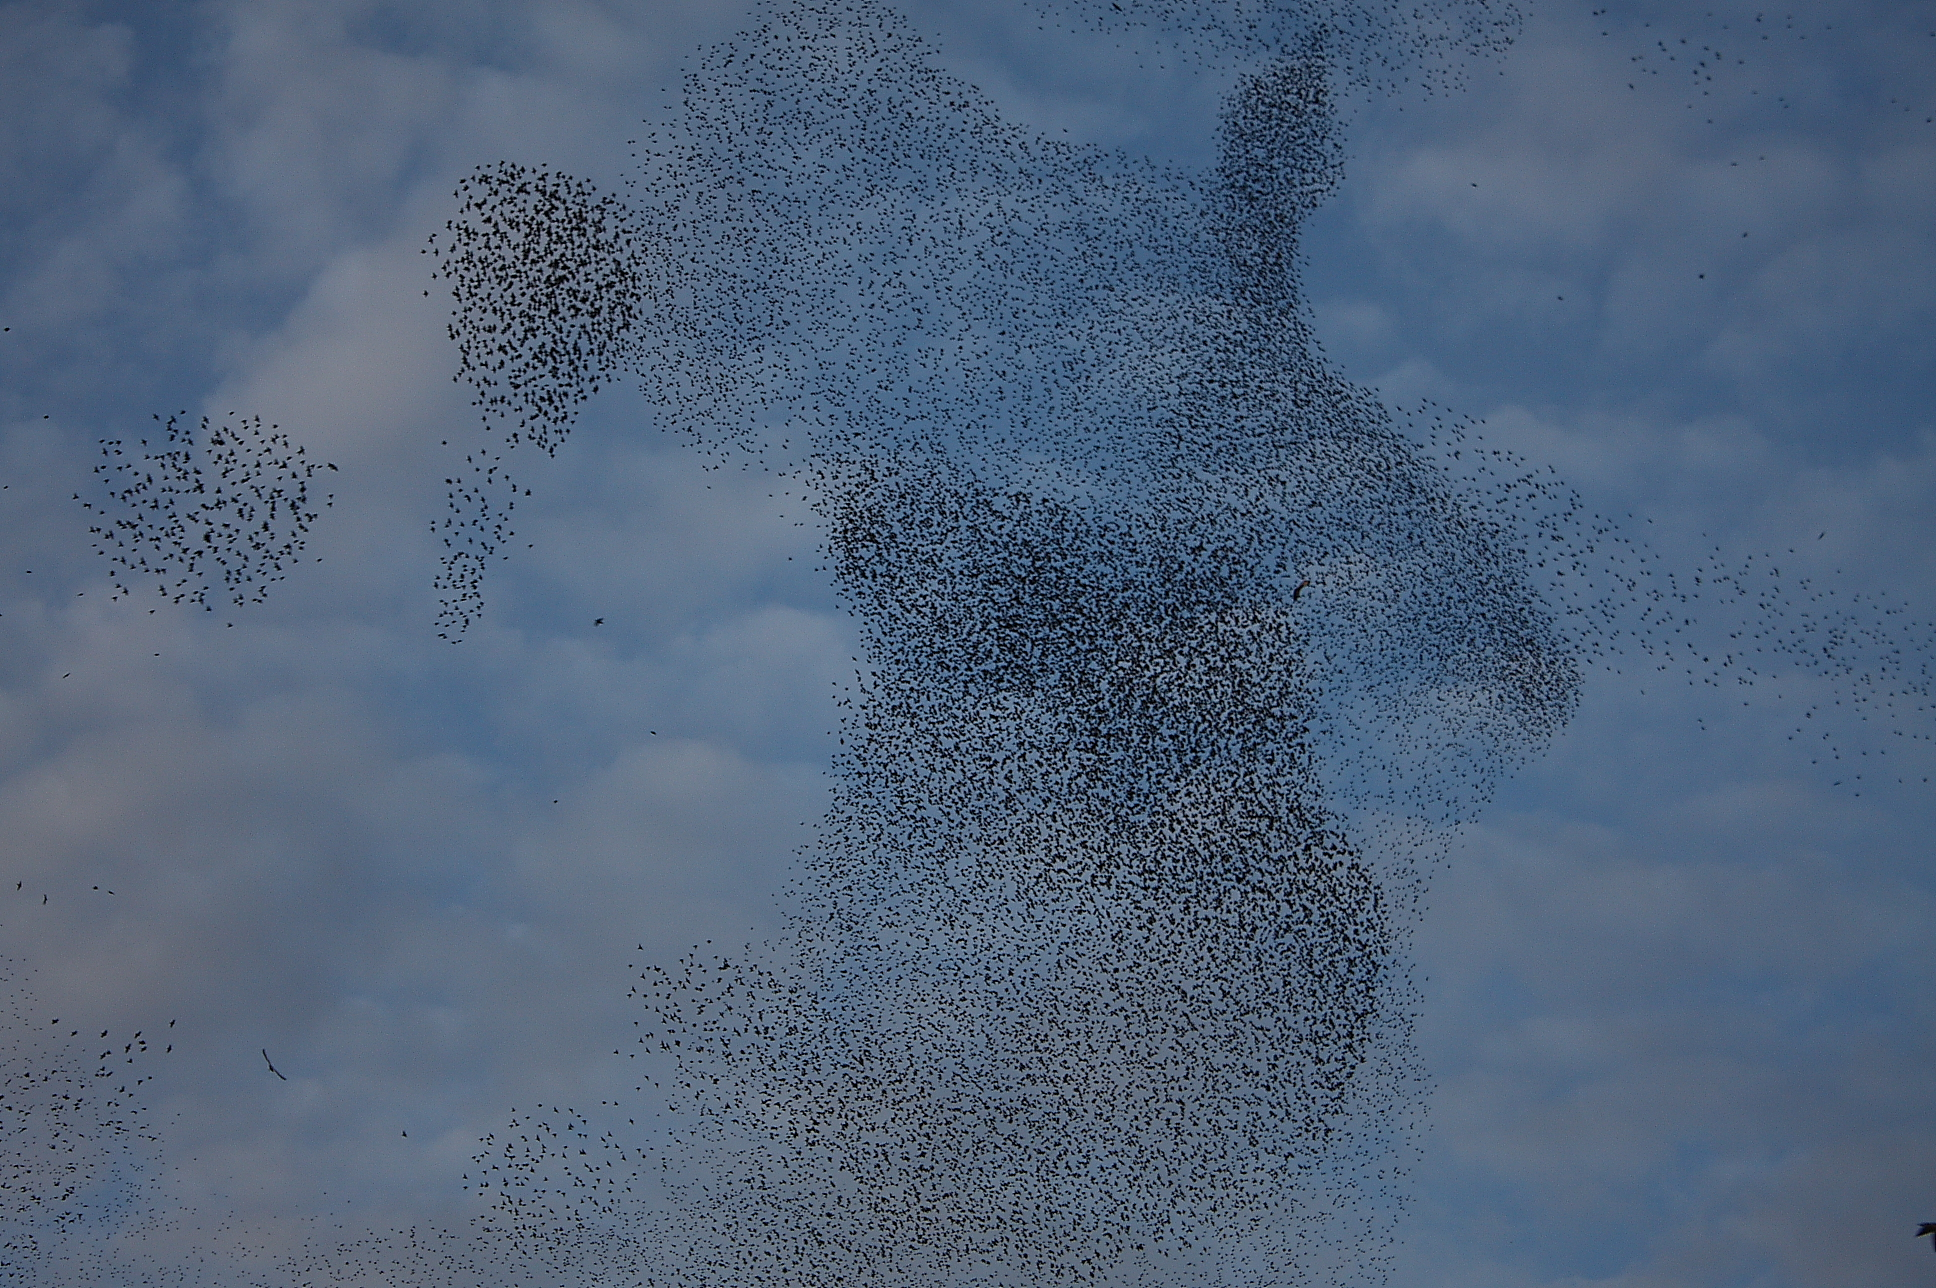
\includegraphics[width=0.95\textwidth]{danza_degli_storni.jpg}
  \begin{center}
    {\large ``La danza degli storni''}\par
    Foto di \_Peck\_\par
    \url{http://www.flickr.com/photos/_pek_/4113244536/}\par
    Licenza: Creative Commons Attribution 2.0\par
  \end{center}
\newpage


\section{Generalità sulle trasformazioni geometriche piane}

\subsection{Introduzione e definizioni}

\begin{quote}
<<C'è una cosa straordinaria da vedere a Roma in questa fine d'autunno ed è il cielo gremito d'uccelli. Il terrazzo del signor Palomar è un buon punto d'osservazione\ldots{} Nell'aria viola del tramonto egli guarda affiorare da una parte del cielo un pulviscolo minutissimo, una nuvola d'ali che volano\ldots{} Quando si pensa agli uccelli migratori ci si immagina di solito una formazione di volo molto ordinata e compatta\ldots{} Questa immagine non vale per gli storni, o almeno per questi storni autunnali nel cielo di Roma\ldots{}>>

\hfill{}Da ``Palomar'', Italo Calvino
\end{quote}

Il volo di questi uccelli disegna nel cielo figure in continua trasformazione, come potete vedere nelle foto. 

Il concetto di trasformazione assume significati diversi a secondo dell'ambito in cui è definito: ad esempio in zoologia la trasformazione di un animale dallo stadio di larva allo stadio di adulto è più propriamente chiamata ``metamorfosi''. Ciò provoca un cambiamento totale del corpo del giovane e l'adulto quasi sempre avrà una forma molto differente da quella della larva.

Il gioco del tangram (pagina~\pageref{tangram}) si basa sulla capacità di passare da una figura ad un'altra senza che nessun pezzo del quadrato base venga tagliato o modificato nelle sue dimensioni: le figure che si ottengono hanno forme diverse, ma sono costituite dagli stessi pezzi. Possiamo dire che sono trasformate le une nelle altre grazie alla nostra fantasia.
 
In geometria si definiscono le trasformazioni come particolari corrispondenze aventi come dominio e codominio il piano considerato come insieme di punti e precisamente si enuncia la

\begin{definizione}
Si definisce \emph{trasformazione geometrica piana} una corrispondenza biunivoca tra punti del piano.
\end{definizione}

Attraverso una legge ben definita, una trasformazione geometrica piana associa ad un punto $P$ del piano uno e un solo punto $P'$ dello stesso piano e, viceversa, il punto $P'$ risulta essere il corrispondente di un solo punto $P$ del piano. Diciamo che $P'$ è l'\emph{immagine di $P$} nella trasformazione.

Indicata con $\Phi$ la legge della corrispondenza, per esprimere il legame tra $P$ e $P'$ scriveremo $\Phi:P\rightarrow P'$ o anche $P\overset{\Phi}{\rightarrow}P'$ e leggeremo: ``$\Phi$ fa corrispondere al punto $P$ il punto $P'$'', oppure $\Phi(P)=P'$ e leggeremo: ``$\Phi$ di $P$ è uguale a $P'$'', scrittura che definisce la trasformazione geometrica come funzione del punto preso in considerazione.

\begin{definizione}
La trasformazione $\Phi$ fa corrispondere ad una figura $\Omega$ del piano la figura $\Omega'$ costituita dalle immagini dei punti della figura iniziale: $\Omega'$ si definisce \emph{immagine di $\Omega$ secondo $\Phi$} e scriveremo $\Phi: \Omega \rightarrow \Omega'$ o anche $\Omega\overset{\Phi}{\rightarrow}\Omega'$ o ancora $\Phi(\Omega)=\Omega'$.
\end{definizione}

Le trasformazioni geometriche che studieremo sono tali da far corrispondere ad una retta $r$ la retta $r'$ individuata dai punti $A'$ e $B'$ immagini di due punti $A$ e $B$ scelti arbitrariamente su $r$. Tali trasformazioni sono chiamate \emph{collineazioni}.

\begin{definizione}
Si chiama \emph{punto unito} o \emph{fisso} nella trasformazione $\Phi$ il punto $P$ che coincide con la sua immagine secondo $\Phi$.
\end{definizione}

Nel caso in cui tutti i punti del piano coincidono con la propria immagine, la trasformazione considerata è detta \emph{identità}.

Per descrivere una trasformazione geometrica è quindi necessario definire come si costruisce l'immagine di un qualunque punto del piano.

\begin{exrig}
\begin{esempio}
Consideriamo nel piano la seguente corrispondenza: fissato un punto $K$ la corrispondenza $S_K$ associa ad ogni punto $P$ del piano il punto $P'$ dello stesso piano tale che $K$ risulti il punto medio del segmento $PP'$. $S_K$ è una trasformazione geometrica?\vspace{7pt}

La definizione è costruttiva:
\[P\overset{S_K}{\rightarrow}P' \wedge PK\cong KP'\text{,} \quad  A\overset{S_K}{\rightarrow}A' \wedge AK\cong KA'\]

Per dimostrare che la corrispondenza è una trasformazione geometrica dobbiamo verificare che si tratta di una corrispondenza biunivoca tra punti del piano: ogni punto ha un corrispondente secondo $S_K$ e, viceversa, ogni punto è immagine di un solo punto del piano stesso. Il punto $K$ è corrispondente di se stesso dunque è un punto unito della trasformazione, anzi è l'unico punto unito (figura~...).

Nella figura~... è rappresentato come opera la trasformazione $S_K$ se applicata ad un quadrato.
\[AK\cong KA'\text{, }BK\cong KB'\text{, }CK\cong KC'\text{, }DK\cong KD'\]

$ABCD\overset{S_K}{\rightarrow}A'B'C'D'$ e i due quadrati hanno le stesse dimensioni.
\end{esempio}

\begin{esempio}
Definiamo la seguente trasformazione geometrica $\Phi$ sul generico punto $P$: dato un punto $O$, tracciamo la semiretta uscente da $O$ e passante per $P$; il punto $P'$, trasformato di $P$ secondo $\Phi$, è il punto della semiretta tale che $OP'=2OP$.\vspace{7pt}

Applicando questa trasformazione al quadrato $ABCD$ (figura~...), il quadrato si trasforma in un altro quadrato ma i due quadrati non hanno le stesse dimensioni.
\end{esempio}
\end{exrig}

Se il piano è dotato di un riferimento cartesiano ortogonale, la legge della trasformazione geometrica piana lega le coordinate di un punto e quelle del suo corrispondente mediante equazioni o sistemi di equazioni.
 
\begin{definizione}
Chiamiamo \emph{equazione della trasformazione} l'insieme delle espressioni algebriche che indicano come si passa dalle coordinate di un generico punto $P$ a quelle della sua immagine $P'$.
\end{definizione}

\begin{exrig}
\begin{esempio}
La corrispondenza $\Phi$ associa ad un punto $P$ del piano dotato di riferimento cartesiano ortogonale il punto $P'$ secondo la seguente legge:
$\Phi : P(x_P;y_P) \rightarrow P'(-2x_P;x_P-y_P)$. La corrispondenza assegnata è una trasformazione geometrica piana?\vspace{7pt}

Strategia risolutiva: 
scegliamo un punto del piano: $P(\ldots{};\ldots{})$ e determiniamo $P'(\ldots{};\ldots{})$;
scegliamo un punto $Q'(\ldots{};\ldots{})$ e determiniamo la controimmagine $Q(\ldots{};\ldots{})$.
posso affermare che la corrispondenza è biunivoca perché \ldots\ldots\ldots\ldots{} e quindi posso affermare che è una trasformazione geometrica.

Applichiamo la stessa trasformazione al quadrato di vertici $A(-1;1)$, $B(-1;3)$, $C(-3;3)$, $D(-3;1)$ (figura~...).
La trasformazione fa corrispondere al quadrato $ABCD$ il parallelogramma $A_1B_1C_1D_1$. Essa ha cambiato la natura della figura geometrica di partenza, ma ha mantenuto il parallelismo tra i lati: $AB\parallel CD \overset{S_K}{\rightarrow} A_1B_1\parallel C_1D_1$, dove $A_1B_1=\Phi(AB)$ e $C_1D_1=\Phi(CD)$.
\end{esempio}
\end{exrig}

Si noti il fatto che esistono trasformazioni geometriche che mantengono invariate forma e dimensioni delle figure a cui sono applicate, altre che mantengono inalterate la forma ma non dimensioni ed altre ancora che non mantengono inalterata neppure la forma.

\begin{definizione}
Si chiamano \emph{proprietà invarianti di una trasformazione} le caratteristiche che una figura e la sua corrispondente mantengono inalterate nella trasformazione.
\end{definizione}

Le principali caratteristiche che una trasformazione può lasciare inalterate sono: la lunghezza dei segmenti, l'ampiezza degli angoli, il rapporto tra segmenti, la misura della superficie, il parallelismo dei segmenti, l'orientamento dei punti del piano, la direzione delle rette, la forma, il numero di lati delle figure.
In questo capitolo tratteremo solo delle trasformazioni che mantengono invariate sia la forma che le dimensioni delle figure.

\begin{definizione}
Si chiama \emph{isometria} una trasformazione piana che associa a due punti distinti $A$ e $B$ del piano i punti $A'$ e $B'$ tali che $AB$ e $A'B'$ risultano congruenti.
\end{definizione}

Solo il primo esempio, tra i precedenti, rappresenta una isometria. Per dimostrare che è una isometria dobbiamo dimostrare che segmenti corrispondenti sono congruenti. Consideriamo il segmento $AP$ e il suo corrispondente $A'P'$; dimostriamo che $AP\cong A'P'$. Considero i triangoli $AKP$ e $A'KP'$, hanno \ldots\ldots\ldots{}\\
Lasciamo al lettore lo sviluppo della dimostrazione.

Riportiamo di seguito le proprietà di una isometria:
\begin{itemize*}
\item L'immagine di una retta è una retta, l'immagine di una semiretta è una semiretta, l'immagine di un segmento è un segmento ad esso congruente.
\item A rette parallele corrispondono rette parallele.
\item A rette incidenti corrispondono rette incidenti.
\item Ad un angolo corrisponde un angolo ad esso congruente.
\end{itemize*}

\begin{definizione}
In una isometria $\Sigma$, una \emph{retta} è \emph{unita} se coincide con la sua immagine, cioè ogni punto della retta data ha come corrispondente un punto della stessa retta.
\end{definizione}

Può succedere che ogni punto di una retta sia un punto unito: in tal caso la retta unita è luogo di punti uniti o \emph{retta fissa}.

$A\in r \wedge B\in r$

$\Sigma : (A\rightarrow A') \wedge (B\rightarrow B')$  $r\equiv r'$

$A'\in r \wedge B'\in r$


$A\in r \wedge B\in r$

$\Sigma : (A\rightarrow A') \wedge (B\rightarrow B')$  $r\equiv r'$

$A'\equiv A \wedge B'\equiv B$



\section{Le isometrie}

Riprendiamo la definizione del paragrafo precedente: si chiama isometria una trasformazione piana che associa a due punti $A$ e $B$ del piano i punti $A'$ e $B'$ tali che $AB\cong A'B'$.

Richiamiamo anche le proprietà:
\begin{itemize*}
\item l'immagine di una retta è una retta, l'immagine di una semiretta è una semiretta, l'immagine di un segmento è un segmento ad esso congruente;
\item a rette parallele corrispondono rette parallele;
\item a rette incidenti corrispondono rette incidenti;
\item ad un angolo corrisponde un angolo ad esso congruente.
\end{itemize*}

Ci proponiamo di studiare particolari isometrie.

\subsection{La simmetria centrale}

\begin{definizione}
Fissato nel piano un punto $K$, chiamiamo \emph{simmetria centrale di centro $K$} (indicata col simbolo $S_K$) la  corrispondenza che associa ad un punto $P$ del piano il punto $P'$ tale che $K$ risulti il punto medio del segmento $PP'$.
\end{definizione}

Per determinare l'immagine di un segmento basta determinare l'immagine dei suoi estremi. Nella figura~... è illustrato come agisce $S_K$ su una qualunque figura piana: l'immagine del triangolo $BCD$ è il triangolo $B'C'D'$ ottenuto determinando l'immagine di ciascuno dei suoi vertici.

\begin{teorema}\label{teo:8.1}
$S_K$ è una isometria.
\end{teorema}

Fissato $K$, centro di simmetria, per la dimostrazione servitevi della figura~ ... 2.

\noindent Ipotesi: $A\overset{S_K}{\rightarrow}A'$, $P\overset{S_K}{\rightarrow}P'$, $PK\cong P'K$, $AK\cong A'K$.\\
Tesi: $AP\cong A'P'$.

Lasciamo al lettore la dimostrazione.

\begin{teorema}\label{teo:8.2}
Rette corrispondenti in $S_K$ sono parallele.
\end{teorema}

\begin{proof}
Osserviamo che per determinare l'immagine $r'$ di una retta $r$ in $S_K$ basta costruire l'immagine $A'$ e $B'$ di due suoi punti $A$ e $B$. Per la costruzione effettuata si ha $AK\cong KA'$ e $BK\cong B'K$. Per il teorema~\ref{teo:8.1} abbiamo $AKB\cong A'KB'$ dunque, in particolare, $A\widehat{B}K\cong A'\widehat{B'}K$. Questi sono angoli alterni interni delle rette $r$ ed $r'$ con trasversale $BB'$, che pertanto risultano parallele.
\end{proof}

\subsubsection{Gli elementi uniti}
\begin{itemize*}
\item l'unico punto unito è il centro di simmetria;
\item sono unite tutte le rette passanti per il centro di simmetria.
\end{itemize*}
Lasciamo al lettore la verifica di quest'ultima proposizione

Immaginate di percorrere il contorno di un triangolo $ABC$ partendo dal vertice $A$ procedendo in ordine alfabetico: state ruotando in senso orario o antiorario? \ldots\ldots{} In quale senso percorrete il contorno di $A'B'C'$ (triangolo trasformato di $ABC$ secondo $S_K$) partendo da $A'$? \ldots\ldots{}

Questo fatto ci permette di concludere che $S_K$ mantiene l'orientamento dei punti: è una \emph{isometria diretta}.

\begin{exrig}
\begin{esempio}
Nel rettangolo $ABCD$ indicate con $O$ il punto di incontro delle diagonali; determinate l'immagine di $ABCD$ nella simmetria di centro $O$. Completate: $S_O:ABCD \rightarrow \ldots\ldots{}$ pertanto il rettangolo è una figura unita nella simmetria avente come centro il punto di intersezione delle sue diagonali.
Vale la stessa affermazione per qualunque parallelogramma? Perché? \ldots\ldots\ldots{}
\end{esempio}
\end{exrig}

\begin{definizione}
Si dice che una figura $F$ ha un \emph{centro di simmetria} se esiste nel piano un punto $K$ tale che nella simmetria di centro $K$, $F$ coincide con la sua immagine $F'$, ovvero $F$ è unita in $S_K$. 
\end{definizione}

\subsubsection{Descrizione analitica di una simmetria centrale}

\begin{definizione}
Fissate le coordinate del centro di simmetria, chiamiamo \emph{equazione di una simmetria centrale} le relazioni che legano le coordinate del generico punto $P$ con le coordinate della sua immagine $P'$. (già data precdentemente) ???
\end{definizione}

Sia $K(x_K;y_K)$ il centro di simmetria e $P(x;y)$ il generico punto di cui vogliamo determinare il corrispondente $P'(x';y')$. Ricordiamo la definizione di simmetria centrale: $K$ risulta il punto medio di $PP'$. Sappiamo che le coordinate del punto medio $M$ di un segmento $AB$ si ottengono dalle coordinate dei suoi estremi $M=\left(\dfrac{x_A+x_B}{2};\dfrac{y_A+y_B}{2}\right)$; nel nostro caso si dovrà avere $x_K=\dfrac{x+x'}{2}$ e $y_K=\dfrac{y+y'}{2}$ da cui possiamo ricavare l'equazione cercata: le coordinate del punto immagine $P'(x',y')$ sono date dall'equazione
\[\begin{cases}x'=2x_K-x\\y'=2y_K-y\end{cases}.\]

\begin{exrig}
\begin{esempio}
Determinare il simmetrico di $P(-1;3)$ nella simmetria centrale di centro $K(1;-1)$.\vspace{7pt}

Riportiamo $K$ e $P$ nel riferimento cartesiano ortogonale e scriviamo l'equazione della simmetria
\[\begin{cases}x'=2-x\\y'=-2-y\end{cases}.\]
Determiniamo le coordinate di $P'$: $x'=2+1=3$ e $y'=-2-3=-5$. Quindi $P'(3;-5)$.
\end{esempio}
\end{exrig}

\subsection{La simmetria assiale}

Ricordiamo la definizione di asse di un segmento, <<l'asse di un segmento $AB$ è la retta perpendicolare al segmento nel suo punto medio $M$>> e studiamo una nuova corrispondenza tra punti del piano.

\begin{definizione}
Fissata nel piano una retta $k$, chiamiamo \emph{simmetria assiale di asse $k$} (indicata col simbolo $S_k$) la corrispondenza che associa ad un punto $P$ del piano il punto $P'$ tale che $k$ risulti l'asse del segmento $PP'$.
\end{definizione}

Per costruire il corrispondente di un punto $P$ del piano procedete con i seguenti passi:
\begin{enumerate*}
\item fissate l'asse di simmetria $k$;
\item prendete un punto $P$ del piano non appartenente a $k$;
\item da $P$ tracciate la perpendicolare $p$ all'asse $k$ e ponete $M=p\cap k$;
\item il corrispondente $P'$ di $P$ si trova su $p$ nel semipiano opposto e $P'M\cong PM$.
\end{enumerate*}

Avrete costruito una figura simile a quella a fianco.

Lasciamo al lettore le verifiche delle seguenti affermazioni circa gli elementi uniti di questa trasformazione $S_k$.
\begin{itemize*}
\item ogni punto dell'asse $k$ è unito;
\item l'asse $k$ è luogo di punti uniti, ossia è una retta fissa;
\item sono unite tutte le rette perpendicolari all'asse $k$;
\end{itemize*}

\begin{teorema}\label{teo:8.3}
La trasformazione $S_k$ è una isometria.
\end{teorema}

Strategia risolutiva:
Dovrete dimostrare che l'immagine di un segmento $AB$ è il segmento $A'B'$ tale che $A'B'\cong AB$; servitevi della figura~... per la dimostrazione, ma prima indicate ipotesi e tesi ($A'B'\cong AB$).
Suggerimento: tracciate la distanza da $A$ e da $A'$ a $BB'$ e dimostrate la congruenza dei triangoli ottenuti.

\begin{teorema}\label{teo:8.4}
Se $r$ è una retta del piano che interseca l'asse $k$ in $R$ allora la sua immagine $r'$ in $S_k$ passa per $R$. $k$ risulta inoltre la bisettrice dell'angolo di vertice $R$ avente come lati $r$ ed $r'$.
\end{teorema}

\noindent Ipotesi: $k$ asse di simmetria, $R=r\cap k$.\\
Tesi: $R=r'\cap k$, $r\widehat{R}k\cong k\widehat{R}r'$.

\begin{proof}
Per costruire $r'$ costruiamo i simmetrici in $S_k$ di due punti scelti su $r$. Possiamo usare il punto $R$ e poi un altro qualunque $A$. Si ottiene $S_k: R \rightarrow \ldots{}$ perché \ldots\ldots\ldots\ldots{} e $S_k: A \rightarrow \ldots{}$

Congiungendo i punti immagine si ottiene $r'$. Concludete \ldots\ldots\ldots\ldots{}
E continuate dimostrando la seconda tesi richiesta.
\end{proof}

\begin{teorema}\label{teo:8.5}
Se $r$ è parallela all'asse di simmetria $k$ allora anche $r'$ risulta parallela a tale asse.
\end{teorema}

Lasciamo la sua dimostrazione al lettore.

Percorrete il contorno del triangolo $ABC$ seguendo l'ordine alfabetico delle lettere ai vertici: il percorso è stato in senso orario/antiorario? Cosa succede percorrendo il contorno del triangolo immagine $A'B'C'$ secondo $S_k$?

Questo fatto ci permette di concludere che $S_k$ non mantiene l'orientamento dei punti: è una \emph{isometria invertente}.

\subsubsection{Descrizione analitica di una simmetria assiale}

\begin{definizione}
Fissata nel riferimento cartesiano ortogonale una retta $k$, chiamiamo \emph{equazione della simmetria assiale di asse $k$} ($S_k$) le relazioni che legano le coordinate del punto $P$ con le coordinate della sua immagine $P'$.
\end{definizione}

Limitiamo la ricerca dell'equazione della simmetria assiale fissando come asse particolari rette; proseguendo negli studi saprete determinare l'equazione di una simmetria assiale il cui asse è una qualunque retta del piano cartesiano.

\paragraph{Simmetria rispetto agli assi coordinati}
~

\begin{exrig}
\begin{esempio}
Studiare la corrispondenza tra punti del piano cartesiano espressa dal seguente predicato: $\Phi:P(x_P;y_P) \rightarrow P'(x_P;-y_P)$.\vspace{7pt}

Completate la tabella: 
\begin{center}
\begin{tabular}{cccc}
\toprule
$x$ & $y$ & $x'$ & $y'$\\
\midrule
$-3$ & $1$ &  &  \\
$0$ & $-2$ &  &  \\
$1$ & $0$ & &  \\
$4$ & $5$ & &  \\
\bottomrule
\end{tabular}
\end{center}

e rappresentate nel riferimento cartesiano ciascun punto e il suo corrispondente.

Completate: $\begin{cases}x'=\ldots{} \\ y'=\ldots{}\end{cases}$.

Motivate la verità delle seguenti proposizioni:\\
<<Ogni punto del piano ha un unico corrispondente>> \ldots\ldots\ldots\ldots\ldots\ldots{}\\
<<Di ogni punto del piano si può determinare la controimmagine>>\ldots\ldots\ldots\ldots\ldots\ldots{}\\
<<La corrispondenza $\Phi$ è una trasformazione geometrica>> \ldots\ldots\ldots\ldots\ldots\ldots{}\\
<<I punti dell'asse $x$ sono uniti>> \ldots\ldots\ldots\ldots\ldots\ldots{}\\
<<La corrispondenza $\Phi$ è una isometria>> \ldots\ldots\ldots\ldots\ldots\ldots{}
\end{esempio}	
\end{exrig}

\begin{definizione}
L'isometria che associa ad ogni punto $P$ del piano il punto $P'$ avente stessa ascissa e ordinata opposta è la \emph{simmetria assiale di asse $x$} ($S_x$) di equazione
\[\begin{cases}x'=x\\ y'=-y\end{cases}.\]
\end{definizione}
 
Ripetete il procedimento seguito nell'esempio precedente studiando la corrispondenza $\Phi:P(x_P;y_P) \rightarrow P'(-x_P;y_P)$ e concludete la seguente
\begin{definizione}
L'isometria che associa ad ogni punto $P$ del piano il punto $P'$ avente stessa \ldots\ldots\ldots{} e \ldots\ldots\ldots{} opposta è la \emph{simmetria assiale di asse \ldots{}} ($S_{\ldots{}}$) di equazione
\[\begin{cases}x'=\ldots\ldots{}\\ y'=\ldots\ldots{}\end{cases}.\]
\end{definizione}

\paragraph{Simmetria rispetto ad una retta parallela agli assi cartesiani}
~

\begin{exrig}
\begin{esempio}
Fissiamo nel piano dotato di riferimento cartesiano ortogonale la retta parallela all'asse $x$ di equazione $y=3$; ci proponiamo di determinare l'equazione della simmetria assiale $S_{y=3}$ avente come asse tale retta.\vspace{7pt}

Determiniamo l'immagine di $P(2;-1)$; da $P$ tracciamo la retta perpendicolare all'asse $y=3$ e indichiamo con $H$ il loro punto di intersezione. Le coordinate di $H$ sono $(2;3)$; l'immagine di $P$ è $P'(2,y')$ ed è tale che $PH\cong P’H$. Da questa congruenza deduciamo
\[\overline{PH}=\overline{P'H}\:\Rightarrow\:\abs{y_H-y_P} = \abs{ y_{P'}-y_H} \:\Rightarrow\: 3-(-1)=y_{P'}-3 \:\Rightarrow\: y_{P'}=7.\]
Quindi $S_{y=3}:P(2;-1)\rightarrow P'(2;7)$.

Ripetendo il procedimento determinate l'immagine dei seguenti punti $A(1;1)$, $B(4;5)$, $C(-1;0)$ e completate:

\[S_{y=3}:\begin{cases}A(\ldots{};\ldots{}) \rightarrow A'(\ldots{};\ldots{})\\
B(\ldots{};\ldots{}) \rightarrow B'(\ldots{};\ldots{})\\
C(\ldots{};\ldots{}) \rightarrow C'(\ldots{};\ldots{})\\
 \end{cases}\]
\end{esempio}
\end{exrig}

Generalizziamo: vogliamo determinare l'equazione della simmetria avente come asse una retta parallela all'asse $x$ di equazione $y=a$. Sia $P(x;y)$ un generico punto del piano e sia $P'(x';y')$ la sua immagine in $S_{y=a}$. Seguendo il ragionamento dell'esempio possiamo scrivere: $\abs{y-a} = \abs{y'-a}$ essendo $P$ e $P'$ da parte opposta rispetto all'asse si ottiene $y-a=-y'+a\:\Rightarrow\: y'=-y+2a$; concludendo $S_{y=a}:P(x;y)\rightarrow P'(x;-y+2a)$ o anche $S_{y=a}:\begin{cases}x'=x\\ y'=-y+2a \end{cases}$.

Verificate, con l'applicazione dell'equazione trovata, i risultati dell'esercizio precedente.

\begin{exrig}
\begin{esempio}
Fissiamo nel piano dotato di riferimento cartesiano ortogonale la retta parallela all'asse $y$ di equazione $x=-1$; ci proponiamo di determinare l'equazione della simmetria assiale $S_{x=-1}$ avente come asse tale retta. Determiniamo l'immagine di $P(2;-1)$; da $P$ tracciamo la retta perpendicolare all'asse $x=-1$ e indichiamo con $H$ il loro punto di intersezione. Le coordinate di $H$ sono $(-1;-1)$; l'immagine di $P$ è $P'(x';-1)$ tale che $PH\cong P'H$. Da questa congruenza deduciamo
\[\overline{PH}=\overline{P'H}\:\Rightarrow\:\abs{x_P-x_H}=\abs{x_H-x_{P'}}\:\Rightarrow\:\abs{2-(-1)}=\abs{-1-x_{P'}}\:\Rightarrow\:x_{P'}=-4.\]
Quindi $S_{x=-1}:P(2;-1)\rightarrow P'(-4;-1)$.

Ripetendo il procedimento, determinate l'immagine dei seguenti punti $A(1;1)$, $B(-3;-2)$, $C(2;0)$ e completate:

\[S_{x=-1}:\begin{cases}A(\ldots{};\ldots{}) \rightarrow A'(\ldots{};\ldots{})\\
B(\ldots{};\ldots{}) \rightarrow B'(\ldots{};\ldots{})\\
C(\ldots{};\ldots{}) \rightarrow C'(\ldots{};\ldots{})\\ \end{cases}\]
\end{esempio}
\end{exrig}

Generalizziamo: vogliamo determinare l'equazione della simmetria avente come asse una retta parallela all'asse $y$ di equazione $x=b$; sia $P(x;y)$ un generico punto del piano e sia $P'(x':y')$ la sua immagine in $S_{x=b}$. Seguendo il ragionamento dell'esempio possiamo scrivere $\abs{x-b}=\abs{b-x'}$, ed essendo $P$ e $P'$ da parte opposta rispetto all'asse si ottiene $x-b=-x'+b:\Rightarrow\: x'=-x+2b$; concludendo, $S_{x=b}:P(x;y)\rightarrow P'(-x+2b;y)$ o anche $S_{x=b}:\begin{cases}x'=-x+2b\\y'=y \end{cases}$


\paragraph{Simmetria rispetto alle bisettrici dei quadranti}
~

\begin{exrig}
\begin{esempio}
Determinate il punto medio $M$ del segmento avente per estremi i punti $P(4;2)$ e $P'(2;4)$ e verificate che il triangolo $POP'$ è isoscele sulla base $PP'$. 
La retta $OM$ è l'asse di simmetria del triangolo considerato. Vero o falso? 
Considerate un'altra coppia di punti $Q(-1;-3)$ e $Q'(-3;-1)$ e ripetete le richieste precedenti.
L'asse $OM$ è la bisettrice del I°-III° quadrante, di equazione $y=x$.
\end{esempio}
\end{exrig}

Generalizziamo: verificate che due punti $P(x_P;y_P)$ e $P'(y_{P};x_{P})$ sono equidistanti dall'origine del riferimento e che il punto medio del segmento $PP'$ appartiene alla retta $y=x$.

\begin{definizione}
La \emph{simmetria assiale} avente come asse la \emph{bisettrice del I\textsuperscript{o}-III\textsuperscript{o} quadrante}, indicata con $S_{b1}$, associa ad ogni punto $P(x_P;y_P)$ il punto $P'(y_P)$ ottenuto scambiando le coordinate di $P$; la sua equazione è $S_{b1}:\begin{cases}x'=y\\y'=x \end{cases}$.
\end{definizione}

Tracciata nel riferimento la retta $y=-x$, dopo aver verificato che è la bisettrice del II\textsuperscript{o}-IV\textsuperscript{o} quadrante, possiamo dare la seguente

\begin{definizione}
La \emph{simmetria assiale} avente come asse la \emph{bisettrice II\textsuperscript{o}-IV\textsuperscript{o} quadrante}, indicata con $S_{b2}$, associa ad ogni punto $P(x_P;y_P)$ il punto $P'(-y_P;-x_P)$ ottenuto scambiando l'opposto delle coordinate di $P$; la sua equazione è $S_{b2}:\begin{cases}x'=-y\\y'=-x \end{cases}$.
\end{definizione}

\begin{comment}
 40   Determinate l’immagine del quadrilatero ABCD di vertici A(0,0), B(2,2), C(5,3), D(0,5) nella simmetria.
 41   Nella simmetria  la retta y=-x è fissa o unita?
 42   Motivate la verità della seguente proposizione:” nella simmetria l’immagine dell’asse x è l’asse y”. Viene mantenuto l’orientamento dell’ asse x?
Completate: : (asse x)(asse …..) e (asse y)(……….) 
Analogamente:  (asse x)(…. …..) e (……..)(……….)
 43   Dato il quadrilatero ABCD di vertici A(0,0), B(3,1), C(4,4), D(1,3), trovate il suo corrispondente in . Quale delle seguenti affermazioni ritenete corretta:
[A] il quadrilatero è fisso nella simmetria considerata,
[B] il quadrilatero è unito nella simmetria considerata.
 44   Determinate il corrispondente del parallelogrammo ABCD di vertici A(-5,1); B(-2,6); C(3,6); D(0,1) in C; perché AA’,BB’, CC’ DD’ sono paralleli? Ricordando che il parallelogrammo ha un centro di simmetria, determinate il centro di simmetria di ABCD e verificate che in  esso ha come immagine il centro di simmetria di A’B’C’D’.


 45   Nel piano cartesiano sono assegnati i punti A(0,3), B(-2,0), C(-1,-3).
1. Determinate i punti A’, B’, C’ immagine in 
2. Calcolate l’area del quadrilatero A’B’C’O, essendo O l’origine del riferimento
3. Motivate la verità della proposizione : “i segmenti AB e A’B’ si incontrano in un punto P della bisettrice II°-IV° quadrante”
4. È vero che AP’B è congruente a PAB’?
 46   Sono assegnate le simmetrie 
Usando qualche punto scelto arbitrariamente riconosci ciascuna di esse e completa la tabella sottostante:
SIMMETRIA
TIPO
CENRO: coordinate
ASSE: equazione
S1 



S2



S3



S4



 47   Quale tra le seguenti caratteristiche è invariante in una simmetria assiale?
[A] la posizione della figura
[B] la direzione della retta
[C] il parallelismo
[D] l’orientamento dei punti
[E] dipende dall’asse di simmetria
 48   I segmenti AB e A’B’ si corrispondono nella simmetria di asse r; sapendo che ABB’A’ è un rettangolo, quale proposizione è vera?
[A] AB è perpendicolare ad r
[B] AB è parallelo ad r
[C] AB appartiene ad r
[D] AB è obliquo rispetto ad r e ABr=H
 49   È assegnato il punto ; determinate il suo corrispondente nelle simmetrie indicate e completate:

 50   Un segmento unito in è
[A] un segmento perpendicolare alla bisettrice I°-III° quadrante
[B] un segmento perpendicolare alla bisettrice II°-IV° quadrante nel suo punto medio
[C] un segmento parallelo alla bisettrice I°-III° quadrante
[D] un segmento perpendicolare alla bisettrice II°-IV° quadrante
[E] un segmento avente il suo punto medio appartenente alla bisettrice II°-IV° quadrante
\end{comment}

\subsection{La traslazione}

\begin{definizione}
Fissato nel piano un vettore $\vec{v}$ si chiama \emph{traslazione di vettore $\vec{v}$} (indicata con $T_{\vec{v}}$) la corrispondenza che ad ogni punto $P$ del piano fa corrispondere il punto $P'$ dello stesso piano in modo che $\vec{PP'}\equiv\vec{v}$.
\end{definizione}

Per costruire il corrispondente di un punto $P$ del piano procedete con i seguenti passi:
\begin{enumerate*}
\item fissate un vettore $\vec{v}$;
\item prendete un punto $P$ del piano;
\item da $P$ tracciate la retta $a$ avente la stessa direzione di $\vec{v}$;
\item su $a$ fissate il punto $P'$ tale che $\vec{PP'}$ sia equipollente a $\vec{v}$.
\end{enumerate*}
Il punto $P'$ così determinato è l'immagine di $P$ nella traslazione, cioè $T_{\vec{v}}:P\rightarrow P'$.

\subsubsection{Gli elementi uniti}

\begin{itemize*}
\item <<Nella traslazione non ci sono punti uniti>>.
\item <<Una retta parallela al vettore che individua la traslazione è unita>>.
\end{itemize*}

Lasciamo al lettore la verifica delle proposizioni enunciate.

\begin{teorema}
La trasformazione $T_{\vec{v}}$ è una isometria.
\end{teorema}

Strategia risolutiva: dimostrate che l'immagine di un segmento $AB$ è un segmento $A'B'$ tale che $AB\cong A'B'$.

\begin{teorema}
Se $r$ ed $r'$ sono due rette corrispondenti in $T_{\vec{v}}$, allora sono parallele.
\end{teorema}

Lasciamo al lettore la dimostrazione del teorema.

\subsubsection{Descrizione analitica di una traslazione}

Pensiamo il piano, dotato di riferimento cartesiano ortogonale, come formato da due cartoncini sovrapposti: sul piano $D$, trasparente, i punti sono rappresentati dal solito simbolo, sull'altro, $C$, sottostante, i punti sono rappresentati con il simbolo ``+''.
Studiamo la corrispondenza $T_{\vec{v}}$ tra i punti del piano $D$ e i punti del piano $C$ espressa dalla legge
\[P(x_P;y_P)\in D \overset{T_{\vec{v}}}\rightarrow P'(x_P+1;y_P+(-3))\in C.\]

Se $P(1;5)$ è un punto di $D$ il suo corrispondente è $P'(2;2)$. Determinate il corrispondente di ciascuno dei seguenti punti $F(0;2)$, $H(-1;8)$, $K(3;3)$ e $V(4;-1)$.

Congiungete ciascun punto $F$, $H$, $K$ e $V$ con il proprio corrispondente $F'$, $H'$, $K'$ e $V'$. I vettori $\vec{FF'}$, $\vec{HH'}$, $\vec{KK'}$ e $\vec{VV'}$ sono equipollenti?

Rispondente alle seguenti domande
\begin{itemize*}
\item \`E vero che il dominio della corrispondenza coincide con $D$?
\item \`E vero che la corrispondenza assegnata è univoca?
\item Si può affermare che è biunivoca?
\item Di quale punto è immagine il punto $S'(0;-4)$?
\item \`E vero che la trasformazione è una isometria?
\end{itemize*}

\begin{comment}
51   Nel piano sono assegnati i tre punti A, B, A’; il punto A’ è immagine di A in una traslazione; dopo aver determinato il vettore della traslazione costruite l’immagine del triangolo ABA’. (figura1)
52   Determinate l’immagine del parallelogrammo ABCD nella traslazione di vettore .
53   Dati due punti distinti A e B e il vettore  della figura 2, detti A’ e B’ i punti immagine di A e B nella traslazione di vettore , rispondete alle questioni:
[A] di che natura è il quadrilatero ABB’A’ ?
[B] può succedere che il quadrilatero in questione sia un rettangolo? E un rombo?
[C] cosa succede se AB è parallelo al vettore ?
54   Come dobbiamo assegnare due segmenti AB e A’B’ perché siano corrispondenti in una traslazione? È unica la traslazione che associa ad AB il segmento A’B’?
\end{comment}

Dagli esercizi precedenti possiamo affermare che la corrispondenza assegnata è una isometria completamente caratterizzata dal vettore $\vec{v}(1;-3)$ pertanto è una traslazione.

\begin{definizione}
Fissato nel riferimento cartesiano ortogonale un vettore $\vec{v}(a;b)$, chiamiamo \emph{equazione della traslazione di vettore $\vec{v}(a;b)$} ($T(a;b)$) le relazioni che legano le coordinate di un generico punto $P$ con quelle della sua immagine $P'$.
\end{definizione}

\begin{definizione}
Siano $(x;y)$ le coordinate del punto $P$ e $(x';y')$ quelle della sua immagine $P'$, l'\emph{equazione della traslazione di vettore $\vec{v}(a;b)$} è $T(a;b):\begin{cases}x'=x+a\\y'=y+b\end{cases}$.
\end{definizione}

\begin{comment}
58   Nel riferimento cartesiano è assegnato il punto P(-4;2); determinate il punto P’ immagine nella traslazione .
Strategia risolutiva:
1. individuate il vettore  della traslazione: 
2. tracciate il vettore nel riferimento cartesiano
3. determinate le coordinate di P’: P’(…;….)
Completate:  è … … … … a ; questo significa che i due vettori hanno … … … direzione (cioè sono … … … …), stesso … … …  e … … … … intensità.
59   Nello stesso riferimento dopo aver fissato un punto Q(…;…) e il punto Q’(…;…) immagine nella stessa traslazione TR(3,-1), dimostrate con le conoscenze di geometria sintetica che PP’Q’Q è un parallelogrammo.
Ipotesi: PP’QQ’; PP’… QQ’                                  
Tesi: … … … 
Dimostrazione:
60   Sappiamo che l’ equazione di una traslazione è . Assegnate le coordinate (x,y) di un punto P e (x’,y’) della sua immagine P’, le componenti del vettore della traslazione sono date da:
[A]			[B]	[C]
[D]			[E]
61   Dopo aver determinato l’equazione della traslazione in cui A’(0,-2) è l’immagine di A(3, 2), determinate il perimetro del triangolo AO’A’ essendo O’ il corrispondente di O(0,0) nella traslazione trovata.
62   Verificate che il punto medio M del segmento PQ di estremi P(-1,4) e Q(5,0) ha come immagine in TR(3,-1) il punto medio M’ del segmento P’Q’. 
63   Applica la traslazione di equazione  al segmento di estremi A(-2;4) B(3;3). 
64   Dati A(1;0) e B(0,2), determina C e D in modo che ABCD sia un quadrato.
65   Determinate l’immagine del triangolo di vertici A(0,2), B(-3,2), C(0,5) nella traslazione TR(4,1); calcolatene perimetro e area.

66   Determinate l’equazione della traslazione di vettore  assegnati dalla figura 3. Determinate inoltre l’immagine del poligono di vertici H(-1,1), K(0,-2), L(3,0), F(1,2).

67   Un vettore  ha modulo unitario, è applicato nell’origine e forma con l’asse delle ascisse un angolo di 30°. Determinate le sue componenti e scrivete l’equazione della traslazione da esso caratterizzata.
\end{comment}

\subsection{La rotazione}

Fissiamo nel piano un angolo convesso di vertice $V$ e lati $a$ e $b$; se immaginiamo, bloccato il vertice $V$, di muovere il lato $a$ fino a farlo sovrapporre al lato $b$ abbiamo ``percorso'' l'angolo muovendoci in senso antiorario; considerando l'angolo concavo di vertice $V$ e lati $a$ e $b$ se immaginiamo, bloccato il vertice $V$, di muovere il lato $a$ fino a farlo sovrapporre al lato $b$ abbiamo ``percorso'' l'angolo concavo muovendoci in senso orario.

\begin{definizione}
Un \emph{angolo} si dice \emph{orientato} quando viene fissato un ordine tra i suoi lati, ad esempio l'ordine alfabetico. Se per andare dal primo lato al secondo ci muoviamo in senso antiorario diciamo che l'angolo è positivo, al contrario avremo un angolo negativo.
\end{definizione}

\begin{exrig}
\begin{esempio}
Nella figura sono disegnati alcuni angoli i cui lati seguono l'ordine alfabetico.
		
\begin{itemize*}
\item Angolo di vertice $A$ e lati $a$ e $b$: $a$ raggiunge $b$ percorrendo l'angolo $\alpha$ in senso antiorario quindi diciamo che $\alpha$ è positivo.
\item Angolo di vertice $G$ e lati $f$ e $g$: $f$ raggiunge $g$ percorrendo l'angolo $\gamma$ in senso orario quindi diciamo che $\gamma$ è negativo.
\item Angolo di vertice $D$ e lati $d$ ed $e$: \ldots\ldots\ldots\ldots\ldots{}
\item Angolo di vertice $T$ e lati $p$ e $t$: \ldots\ldots\ldots\ldots\ldots{}
\end{itemize*}
\end{esempio}
\end{exrig}
		
\begin{definizione}
Fissato un punto $O$ e un angolo orientato $\alpha$ chiamiamo \emph{rotazione di centro $O$ e ampiezza $\alpha$} ($R_{O,\alpha}$) la corrispondenza che associa ad un punto $P$ del piano il punto $P'$ tale che $PO\cong P'O$ e $P\widehat{O}P'=\alpha$.
\end{definizione}
		
Fissato l'angolo orientato $\alpha$, il punto $O$ centro della rotazione, l'immagine del punto $P$ si determina con i seguenti passi:
\begin{enumerate*}
\item congiungiamo $O$ con $P$;
\item tracciamo la circonferenza di centro $O$ e raggio $OP$;
\item costruiamo, con vertice in $O$, l'angolo $\beta\cong \alpha$;
\item $P'$ è il punto di intersezione della circonferenza con il secondo lato $h$ dell'angolo $\beta$.
\end{enumerate*}
		
\begin{comment}		
68   Prendete in considerazione l’angolo  di vertice T, sia O il centro di rotazione e F un punto del piano di cui si vuole determinare l’immagine. Costruite F’ seguendo i passi illustrati sopra.
\end{comment}
		
\subsubsection{Gli elementi uniti}
\begin{itemize*}
\item <<Il centro è l'unico punto unito>>.
\item <<Sono unite tutte le circonferenze aventi il centro nel centro di rotazione>>.
\end{itemize*}
		
Lasciamo al lettore la verifica di quanto affermato.
		
\begin{teorema}
La rotazione è una isometria.
\end{teorema}
		
Per dimostrare il teorema proposto, servitevi della figura a lato, nella quale è segnato il centro di rotazione $O$, l'angolo orientato $\alpha$ ($c$ è il primo lato) e un segmento $BC$.
Strategia risolutiva: costruite l'immagine $B'C'$ nella rotazione assegnata.
		
\noindent Ipotesi: \ldots\ldots\ldots{}\\
Tesi: \ldots\ldots\ldots{}
		
\emph{Dimostrazione.} \ldots\ldots\ldots{}
		
\begin{teorema}
La rotazione è una isometria diretta.
\end{teorema}
		
Ricordate che per questa dimostrazione basta costruire l'immagine di una figura e verificare che viene mantenuto il verso di percorrenza del contorno. Vi proponiamo, nella figura a lato, il centro e l'angolo di rotazione; disegnate una figura geometrica, costruite la sua immagine e concludete.

\begin{comment}		
69   Costruite l’immagine del quadrato ABCD nella rotazione di +90° avente come centro di simmetria il vertice B.
Fissate i punti medi M ed N rispettivamente di AB e di CD; dove si trovano le rispettive immagini?
70   È vero  che il quadrato è unito nella rotazione avente come centro il punto d’incontro delle diagonali e come ampiezza 90°?
71   “L’ortocentro di un triangolo equilatero è il centro di una rotazione in cui il triangolo è unito”. Determinate l’angolo di rotazione.
72   Costruite l’immagine A’B’C’ del triangolo equilatero ABC nella rotazione di centro B e ampiezza . Dimostrate che C, B, A’ sono allineati e che ABC’ è un triangolo equilatero congruente a quello dato.
\end{comment}
		
\section{Composizione di isometrie}
		
\subsection{Composizione di isometrie di tipo diverso}
		
\begin{exrig}
\begin{esempio}
Riferendovi alla figura, completate:
		
Nel riferimento cartesiano ortogonale sono assegnati il triangolo $EFD$ avente i vertici di coordinate $D(\ldots{};\ldots{})$, $E(\ldots{};\ldots{})$ ed $F(\ldots{};\ldots{})$ e il vettore $\vec{u}$ di componenti (\ldots{};\ldots{}). Con la traslazione di vettore $\vec{u}$ si ha $DEF \overset{T_{\vec{u}}}\rightarrow \ldots\ldots\ldots{}$ e $DEF\cong D'E'F'$ essendo la traslazione una isometria.
		
Nel piano è tracciata la retta a di equazione $x=3$; nella simmetria assiale $S_{x=3}$ si ha $D'E'F' \overset{S_{x=3}}\rightarrow \ldots\ldots\ldots{}$ e $D'E'F'\cong D''E''F''$ essendo la simmetria assiale una isometria.
		
Completate con le coordinate dei punti
		
\[\left.\begin{array}{l}D(\ldots{};\ldots{}) \overset{T_{\vec{u}}}\rightarrow D'(\ldots{};\ldots{})\overset{S_{x=3}}\rightarrow D''(\ldots{};\ldots{})\\
E(\ldots{};\ldots{}) \overset{T_{\vec{u}}}\rightarrow E'(\ldots{};\ldots{})\overset{S_{x=3}}\rightarrow E''(\ldots{};\ldots{})\\
F(\ldots{};\ldots{}) \overset{T_{\vec{u}}}\rightarrow F'(\ldots{};\ldots{})\overset{S_{x=3}}\rightarrow F''(\ldots{};\ldots{})\end{array} \right\}\text{ e } DEF\overset{T_{\vec{u}}}\rightarrow D'E'F'\overset{S_{x=3}}\rightarrow D''E''F''\]
e $DEF\cong D''E''F''$ per la proprietà transitiva della congruenza.
\end{esempio}
\end{exrig}
		
\begin{definizione}
Chiamiamo \emph{composizione di due isometrie $\Phi_1$ e $\Phi_2$} l'isometria $\Phi = \Phi_2 \circ \Phi_1$ (e leggiamo ``$\Phi_2$ composta con $\Phi_1$''), che associa ad un qualunque punto $P$ del piano il punto $P''$ ottenuto determinando prima l'immagine $P'$ di $P$ in $\Phi_1$ e di seguito l'immagine $P''$ di $P'$ in $\Phi_2$. In formula: $\Phi(P)=\Phi_1 \circ \Phi_2:P\overset{\Phi_1}\rightarrow P' \overset{\Phi_2}\rightarrow P''$.
\end{definizione}

Riprendendo l'esempio precedente concludiamo $DEF \overset{S_{x=3} \circ T_{\vec{u}}}\rightarrow D''E''F''$.
			
In generale, la composizione di isometrie non è commutativa, cioè $\Phi_1\circ\Phi_2 \neq \Phi_2\circ\Phi_1$.
Se, utilizzando l'esempio precedente volete verificare che $S_{x=3}\circ T_{\vec{u}} \neq T_{\vec{u}}\circ S_{x=3}$, troverete un risultato che sembra contraddire quanto affermato; basta però un controesempio per convincerci della verità della proposizione sopra enunciata. 
			
\paragraph{Controesempio}
Determinate l'immagine del punto $P(2;2)$ in $S_y \circ T{\vec{u}}$ essendo $\vec{u}(3;2)$. Quindi confrontarla con l'immagine dello stesso punto in $T{\vec{u}}\circ S_y$.\vspace{7pt}
			
Tracciate il vettore $\vec{u}(3;2)$ e completate
			
\noindent $P(2;2) \overset{T_{\vec{u}}}\rightarrow P'(\ldots{};\ldots{}) \overset{S_y}\rightarrow P''(\ldots{};\ldots{})$\\
$P(2;2) \overset{S_y}\rightarrow P'(\ldots{};\ldots{}) \overset{T_{\vec{u}}}\rightarrow P''(\ldots{};\ldots{})$
			
Concludete: la composizione di isometrie non è \ldots\ldots\ldots{}, infatti si ha $S_y \circ T_{\vec{u}} \ldots{} T_{\vec{u}} \circ S_y$.
			
Possiamo determinare l'equazione che lega le coordinate del punto iniziale con quelle della sua immagine nell'isometria ottenuta dalla composizione? Procediamo per passi:
			
I° passo: scriviamo l'equazione della traslazione $T_{\vec{u}}=\begin{cases}x'=x+3\\y'=y+2\end{cases}$ e della simmetria rispetto all'asse $y$ $S_y=\begin{cases}x'=-x\\y'=y\end{cases}$.
			
II° passo: determiniamo l'immagine di $P(x_P;y_P)$ in $S_y \circ T_{\vec{u}}$:
			
\[P(x_P;y_P)\overset{T_{\vec{u}}}\rightarrow P'(x_P+3;y_P+2) \overset{S_y}\rightarrow P''(-x_P-3;y_P+2)\:\Rightarrow\: S_y\circ T_{\vec{u}}:\begin{cases}x''=-x_P-3\\ y''=y_P+2\end{cases}\]
			
III° passo: determiniamo l'immagine di $P(x_P;y_P)$ in $T_{\vec{u}}\circ S_y$:
			
\[P(x_P;y_P)\overset{S_y}\rightarrow P'(-x_P;y_P) \overset{T_{\vec{u}}}\rightarrow P''(-x_P+3;y_P+2)\:\Rightarrow\: T_{\vec{u}}\circ S_y:\begin{cases}x''=-x_P+3\\ y''=y_P+2\end{cases}\]
			
Dunque confermiamo la non commutatività dell'operazione di composizione delle isometrie.
			
\begin{comment}			
73   Nel piano è assegnato il punto C e il vettore ; costruite l’immagine del punto P nell’isometria  e anche l’immagine dello stesso punto P nell’isometria  .
74   Il centro della simmetria è il punto , il vettore della traslazione è  e il punto di cui vogliamo determinare l’immagine è scelto da voi arbitrariamente. Ripetete l’esercizio precedente e determinate l’equazione di 
75   Sono assegnati il punto C(-4,3), la retta x=1 e il punto P(0,5); determinate l’immagine P” di P nell’isometria  e l’immagine P* di P nell’isometria . È vero che p” e P* si corrispondono nella simmetria ? Determinate l’area del triangolo PP”P*.	(R. area=40u2)
76   È assegnato un punto O; determinate l’immagine P’ di un punto P nella rotazione di centro O e angolo di 60° e l’immagine P” di P’ nella simmetria avente come asse la retta PO. 
1. Completate: 
2. Dimostrate che P, P’, P” appartengono alla circonferenza di centro O e raggio OP
3. Individuate le caratteristiche del quadrilatero PP”OP’
4. Determinatene l’area, supponendo 			(R. )
\end{comment}
			
\subsection{Composizione di isometrie dello stesso tipo}
			
\begin{exrig}
\begin{esempio}
Determinate l'equazione dell'isometria che si ottiene componendo la simmetria che ha per asse l'asse $x$ e quella avente come asse l'asse $y$: $S_y \circ S_x\begin{cases}\ldots\ldots{}\\\ldots\ldots{}\end{cases}$ Quale isometria avete ottenuto?
Determinate l'equazione di $S_x \circ S_y\begin{cases}\ldots\ldots{}\\\ldots\ldots{}\end{cases}$ Cosa potete concludere?\vspace{7pt}
			
Lasciamo al lettore la sua risoluzione.
\end{esempio}
	
\begin{esempio}
Nel riferimento cartesiano ortogonale sono tracciate le rette $a: x=-1$ e $b: y=2$ e il punto $B(2;1)$.
\begin{enumerate*}
\item Determinate l'immagine di $B$ nell'isometria $\Omega_1 = S_a \circ S_b$ della quale indicherete l'equazione.
\item Determinate l'immagine di $B$ nell'isometria $\Omega_2 = S_b \circ S_a$ della quale indicherete l'equazione.
\item Indicate le coordinate del punto $K$ e scrivete l'equazione della simmetria di centro $K$. Cosa concludete?
\end{enumerate*}
			
Lasciamo al lettore la sua risoluzione.
\end{esempio}
\end{exrig}
			
			
Generalizziamo: le rette $a$ e $b$ sono perpendicolari e $O$ è il loro punto di intersezione. Dimostrate che:
\begin{itemize*}
\item La composizione delle due simmetrie di assi $a$ e $b$ è commutativa.
\item L'isometria $\Omega = S_a\circ S_b = \S_b \circ S_a$ è la simmetria centrale di centro $O$.
\end{itemize*}
			
Conclusione: La composizione di due simmetrie assiali con assi perpendicolari in $O$ è la simmetria centrale di centro $O$. L'operazione è commutativa.
			
\begin{exrig}
\begin{esempio}
Determinate l'immagine del punto $P$ nell'isometria ottenuta componendo due simmetrie con assi incidenti $P\overset{S_a}\rightarrow P' \overset{S_b}\rightarrow P''$. Servitevi della figura a lato.
			
Verificate che la composizione non è commutativa determinando $P\overset{S_b}\rightarrow P' \overset{S_a}\rightarrow P''$.
			
Dimostrate che $PS \equiv P'A\equiv P''A\equiv P_1'A \equiv P_1''A$.
Dimostrate che i punti $P$, $P'$, $P''$, $P_1'$ e $P_1''$ stanno sulla circonferenza di centro $A$.
Dimostrate che $P\widehat{A}P''=2\cdot \alpha$
\end{esempio}
\end{exrig}
			
Conclusione: La composizione di due simmetrie assiali con assi incidenti nel punto $A$ è la rotazione di centro $A$ e angolo orientato $2\cdot \alpha$; punti corrispondenti appartengono alla circonferenza di centro $A$ e raggio $PA$. La composizione in esame non è commutativa.

\begin{comment}			
80   ABC è un triangolo equilatero e O è il centro della circonferenza circoscritta. Dimostrate che il triangolo è unito nella rotazione di centro O e angolo =120°. Analogamente il quadrato ABCD  è unito nella rotazione di centro H, punto d’incontro delle sue diagonali, di angolo =90°. 
81   Giustificate la verità della proposizione: “La simmetria centrale di centro K è una rotazione di 180°”.
82   Nel piano dotato di riferimento cartesiano è tracciata la bisettrice I°-III° quadrante e la retta . Completate le osservazioni seguenti:
il punto di intersezione K ha coordinate K(…,…)
l’angolo delle due rette è di …..°
83   Scrivete l’equazione della simmetria avente come asse la bisettrice:  e l’equazione della simmetria di asse la retta : .
84   Determinate le coordinate del punto P” immagine di P, arbitrariamente scelto, in  e scrivete l’equazione di .
Concludete:  è la rotazione di centro ……. e angolo ……(ricordate il segno all’angolo di rotazione)
85   Determinate le coordinate del punto P* immagine di P, arbitrariamente scelto, in  e scrivete l’equazione di *.
Concludete: * è la rotazione di centro ……. e angolo ……(ricordate il segno all’angolo di rotazione)
86   Determinate l’equazione della isometria  e stabilite se esiste qualche elemento unito. Come cambia l’equazione dell’isometria  rispetto alla precedente? Sia J che J* sono rotazioni: determinate centro e angolo (con segno) di ciascuna. A questo scopo potete utilizzare il punto P(2,4) o un punto arbitrariamente scelto.
87   Determinate l’immagine del punto A nell’isometriaessendo a e b le rette parallele segnate in figura e A il punto dato. Dimostrate che  essendo d la distanza tra le rette a e b.
Fissate arbitrariamente un altro punto B non appartenente ad alcuna delle rette date e determinate la sua immagine B” nell’isometria .
È vero che  ? Potete concludere che l’isometria  è la traslazione di vettore ?
\end{comment}
			
\begin{definizione}
La composizione di due simmetrie assiali con assi paralleli è una \emph{traslazione di vettore} avente direzione perpendicolare ai due assi di simmetria e modulo uguale al doppio della distanza tra gli stessi assi.
\end{definizione}
			
\begin{comment}			
88   Verificate che la traslazione  è caratterizzata da un vettore avente modulo e direzione uguali al vettore  trovato nell’esercizio precedente, ma verso opposto.
89   Nel riferimento cartesiano ortogonale sono assegnati i punti A(1,5); B(2,1); C(-1,3). Determinate i punti A”, B”, C” immagine rispettivamente di A, B, C nella traslazione . Scrivete  l’equazione della traslazione, individuate il vettore che la definisce calcolandone modulo e direzione. 
90   Determinate i vettori  delle traslazioni  e il vettore . Verificate che . 
Cosa otteniamo dalla composizione ? Sapresti darne la motivazione?
Concludete: componendo due traslazioni si ottiene ……………………………………….
91   Nel riferimento cartesiano ortogonale Oxy è assegnato il punto ; scrivete l’equazione della simmetria centrale di centro O  e l’equazione della simmetria centrale di centro  . Determinate l’immagine P” del punto  nell’isometria  di cui avrete scritto l’equazione e determinate . Determinate Q” immagine di nell’isometria  e determinate . Potete affermare che ? Verificate che .
			
92   è vero che  sono la stessa isometria?
93   Dimostrate che la composizione di due simmetrie centrali è una traslazione caratterizzata dal vettore parallelo alla retta passante per i due centri e modulo uguale al doppio della loro distanza.
\end{comment}			
			
\begin{definizione}
La composizione di due simmetrie centrali è una \emph{traslazione di vettore} avente la direzione della retta $OO_1$ e modulo uguale al doppio della distanza tra $O$ e $O_1$.
\end{definizione}
			
\begin{comment}			
94   Composizione di due simmetrie assiali con assi paralleli.
Prima simmetria ; Seconda simmetria 
Componendo le due simmetrie si ha  che è … … … … … … … … … 
Se a=b le due simmetrie sono … … … … … … … … … … la loro composizione è … … … … … …
95   Composizione di due simmetrie assiali con assi perpendicolari.
Una simmetria con asse parallelo all’asse y ha equazione  e asse x = a 
Mentre una simmetria con asse parallelo all’asse x ha equazione   e asse y = b 
Componendo le due simmetrie otteniamo … …   
\end{comment}			
			
\subsection{Isometria inversa}
			
Sappiamo che dalla composizione di due isometrie si ottiene una isometria e in generale componendo due trasformazioni geometriche si ottiene una trasformazione geometrica, ossia una corrispondenza biunivoca tra punti del piano.
Considerate due trasformazioni $\Psi_1$ e $\Psi_2$ e detta $I$ l'identità può succedere che $\Psi_1 \circ \Psi_2 = \Psi_2 \circ \Psi_1 = I$ cioè che l'immagine di un generico punto $P$ nella trasformazione composta coincida con $P$ stesso.
			
\begin{definizione}
Si chiama \emph{inversa} di una trasformazione $\Psi$ la trasformazione che composta con $\Psi$, a destra o a sinistra, dà origine all'identità e la indicheremo con $\Psi^{-1}$; in simboli: $\Psi \circ \Psi^{-1} = \Psi^{-1} \circ \Psi = I$.
\end{definizione}
			
\begin{definizione}
Si chiama \emph{involutoria} una trasformazione che coincide con la sua inversa.
\end{definizione}
			
\begin{comment}			
Per quanto riguarda le isometrie studiate
96   Verificate che:
1. l’inversa della traslazione di vettore  è la traslazione di vettore ; 
2. l’inversa di una rotazione di centro O e angolo  è la rotazione di centro O e angolo -
97   Verificate che le simmetrie (centrale, assiale) hanno se stesse come isometria inversa, ossia 
			
98   La proposizione “la simmetria centrale è la composizione di due simmetrie assiali” è:
[A] sempre vera		[B] vera se i due assi sono incidenti 	[C] mai vera
[D] vera se i due assi sono perpendicolari		[E] vera se i due assi sono paralleli
99   Completa la proposizione: “La simmetria centrale di centro  può essere ottenuta come composizione delle due simmetrie assiali di assi le rette … … … … … … e la sua equazione è … … … … … … … … … … … … … … … …
			
100   Stabilite il valore di verità delle proposizioni:
Componendo due isometrie si ottiene una isometria
a) Componendo due simmetrie assiali si ottiene una simmetria assiale				V F
b) Componendo due traslazioni si ottiene una traslazione						V F
c) Componendo due simmetrie centrali si ottiene una simmetria centrale			V F
d) Componendo due simmetrie assiali di assi incidenti si ottiene una rotazione			V F
e) Componendo due rotazioni si ottiene una rotazione						V F
f) L’identità si ottiene componendo una isometria con sé stessa					V F
g) L’inversa di una traslazione è la stessa traslazione						V F
h) Componendo una simmetria centrale con una rotazione si ottiene l’identità			V F
i) Componendo una simmetria centrale di centro H con la simmetria assiale avente come asse una retta passante per H si ottiene sempre l’identità								V F
			
Ulteriori esercizi sulle isometrie
101   L’equazione  descrive: 
			[A] la simmetria di asse l’asse y					[B] la simmetria di asse la retta 	
			[C] la traslazione di vettore 				[D] la simmetria di asse x=2			
			[E] la simmetria di centro C(4,0)
			102   La trasformazione  è un’isometria?
			103   Il segmento di estremi A(3,4) e B(3,-2) ha come simmetrico il segmento di estremi A’(3,2) e B’(5,2); è stata eseguita:
			[A] la simmetria di asse la retta 	
			[B] la simmetria 		
			[C] la simmetria 
			[D] la simmetria di asse la retta 		
			[E] la simmetria 
			104   Attribuisci il valore di verità alle seguenti proposizioni:
			a) In una isometria vi è almeno un elemento unito
			b) Nella simmetria centrale vi sono infinite rette unite, ma solamente un punto unito
			c) In ogni triangolo vi è almeno un asse di simmetria
			d) Qualche quadrilatero ha un centro di simmetria
			e) Il triangolo equilatero ha un centro di simmetria
			f) Il rombo è l’unico quadrilatero avente due assi di simmetria
			g) Tutte le rette aventi la stessa direzione del vettore della traslazione sono rette unite
			h) Solo la simmetria assiale è una isometria invertente
			i) Rette parallele hanno come immagine in una isometria rette parallele
			j) In una isometria una retta è sempre parallela alla sua immagine 
			105   Il quadrilatero di vertici A(5,0), B(9,0), C(12,4), D(7,3) nella simmetria ha fisso il lato AB. Spiegate come sia possibile questo fatto.
			106   Dimostrate che la bisettrice di un angolo è il suo asse di simmetria
			107   Il rettangolo ABCD con AB<BC ha come immagine il rettangolo A’B’C’D’ nella simmetria avente come asse la retta AC. Potete affermare che AB’DCD’B è un esagono regolare?
			
			108   I due segmenti della figura1 possono essere corrispondenti in una simmetria centrale? 
			
			
			
			109   Nella figura abbiamo disegnato il quadrato ABCD e il punto A’ corrispondente di A in una isometria. Stabilite quale isometria è completamente fissata con questi elementi (simmetria assiale, traslazione, simmetria centrale) e determinate in essa l’immagine del quadrato. 
			
			110   Costruite l’immagine di un triangolo rettangolo ABC (non isoscele) di ipotenusa BC
			a) in ciascuna delle simmetrie 
			b) nella simmetria  essendo M il punto medio dell’ipotenusa
			c) in ciascuna delle simmetrie aventi come assi le rette dei lati
			111   Comporre due traslazioni di vettori v1(2; 3) e v2(3; 6) applicandole al triangolo ABC, con A(-2; -1) B(-1; -2) C(-4; -3) . 
			112   Determina il corrispondente A'B' del segmento di vertici A(-2; 6) e B(-3; 3) nella simmetria di asse x=-1, applica poi al segmento ottenuto un'ulteriore simmetria con asse x=4. Utilizzando l’equazione per la composizione di due simmetrie con assi paralleli tra di loro trova le nuove coordinate dei due punti A e B.  
			113   Determina il corrispondente A'B' del segmento di vertici A(1; -6) e B(4; 3) nella simmetria di asse x = 2, applica poi al segmento ottenuto un ulteriore simmetria con asse y = 1. Utilizzando l’equazione per la composizione di due simmetrie con assi perpendicolari tra di loro determina le nuove coordinate dei due punti A e B. 
			114   Componi le seguenti trasformazioni geometriche scrivendo l'equazione della trasformazione composta e fornendo un esempio con disegno relativo. 
			a) Due rotazioni con lo stesso centro 
			b) Due rotazioni con centro diverso 
			c) Due simmetrie centrali 
			d) Due rotazioni di un angolo retto 
			115   Sono assegnate le simmetrie assiali
			
			a) Individuate l'asse di simemtria di ciascuna, rappresentate nel riferimento cartesiano ortogonale i rispettivi assi indicandoli con s1, s2, s3, s4; completate e riproducete nello stesso riferimento
			
			
			b) Siano A, B, C, D i punti ; dimostrate che i triangoli ABC e CDE sono rettangoli isosceli e che i lati dell'uno sono il quadruplo dei lati dell'altro.
			c) Determinate il rapporto tra i loro perimetri e tra le loro aree.
\end{comment}			
			
			
\newpage
			
% Copyright (c) 2015 Daniele Masini - d.masini.it@gmail.com

\section{Esercizi}

\subsection{Esercizi riepilogativi}

\begin{esercizio}
\label{ese:8.1}
Le coppie di figure rappresentate nella figura~\ref{fig:ese8.1} si corrispondono in una trasformazione geometrica piana: associate a ciascuna coppia la caratteristica che rimane immutata nella trasformazione, ossia individuate l'invariante o gli invarianti della trasformazione.
\end{esercizio}

\begin{figure}[!htb]
	\centering% (c) 2014 Daniele Masini - d.masini.it@gmail.com
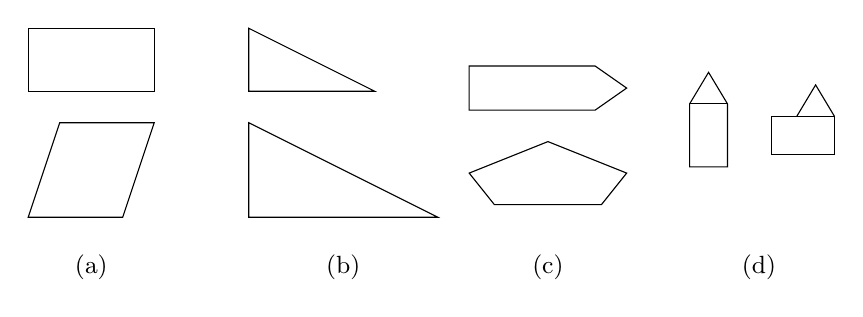
\begin{tikzpicture}[scale=0.8,font=\small]
\usetikzlibrary{calc}

\begin{scope}
\draw (0,0) rectangle (2,1);
\draw (0,-2) -- (1.5,-2) -- (2,-0.5) -- (0.5,-0.5) -- cycle;
\node at (1,-2.8) {(a)};
\end{scope}

\begin{scope}[xshift=3.5cm]
\draw (0,0) -- (0,1) -- (2,0) -- cycle;
\draw (0,-2) -- (0,-0.5) -- (3,-2) -- cycle;
\node at (1.5,-2.8) {(b)};
\end{scope}

\begin{scope}[xshift=7cm]
\begin{scope}[yshift=-0.3cm]
\draw (0,0) -- (0,0.7) -- (2,0.7) -- (2.5,0.35) -- (2,0) -- cycle;
\draw (0,-1) -- (1.25,-0.5) -- (2.5,-1) -- (2.1,-1.5) -- (0.4,-1.5) -- cycle;
\end{scope}
\node at (1.25,-2.8) {(c)};
\end{scope}

\begin{scope}[xshift=10.5cm]
\begin{scope}[yshift=-1.2cm]
\draw (0,0) -- (0,1) -- (0.3,1.5) -- (0.6,1) -- (0.6,0) -- cycle;
\draw (0,1) -- (0.6,1);
\end{scope}
\begin{scope}[xshift=1.3cm, yshift=-1cm]
\draw (0,0) -- (0,0.6) -- (1,0.6) -- (1,0) -- cycle;
\draw (0.4,0.6) -- (0.7,1.1) -- (1,0.6);
\end{scope}
\node at (1.1,-2.8) {(d)};
\end{scope}

\end{tikzpicture}

	\caption{Esercizio~\ref{ese:8.1}}\label{fig:ese8.1}
\end{figure}

\begin{esercizio}
\label{ese:8.2}
Si sa che una trasformazione geometrica muta un quadrato in un rombo; gli invarianti di questa trasformazione sono:
\begin{enumeratea}
\item il parallelismo dei lati e l'ampiezza degli angoli;
\item l'ampiezza degli angoli e la misura dei lati;
\item solo il parallelismo 	dei lati;
\item il parallelismo dei lati e la perpendicolarità delle diagonali.
\end{enumeratea}
\end{esercizio}

\begin{esercizio}
\label{ese:8.3}
Quali coppie rappresentate nella figura~\ref{fig:ese8.3} sono formate da figure corrispondenti in una isometria?
\end{esercizio}

\begin{figure}[!htb]
	\centering% Copyright (c) 2015 Daniele Masini - d.masini.it@gmail.com

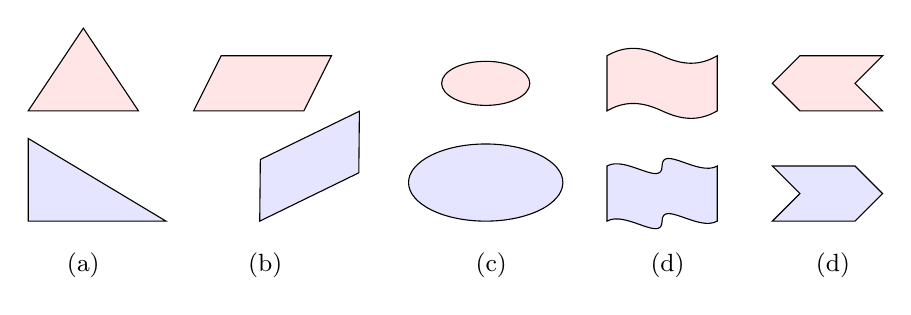
\begin{tikzpicture}[scale=0.7,font=\small]
\usetikzlibrary{calc}

\begin{scope}
\draw[fill=red!10] (0,0) -- (2,0) -- (1,1.5) -- cycle;
\draw[fill=blue!10] (0,-2) -- (0,-0.5) -- (2.5,-2) -- cycle;
\node at (1,-2.8) {(a)};
\end{scope}

\begin{scope}[xshift=3cm]
\begin{scope}
\draw[fill=red!10] (0,0) -- (2,0) -- (2.5,1) -- (0.5,1) -- cycle;
\end{scope}
\begin{scope}[xshift=1.2cm, yshift=-2cm, rotate=26]
\draw[fill=blue!10] (0,0) -- (2,0) -- (2.5,1) -- (0.5,1) -- cycle;
\end{scope}
\node at (1.3,-2.8) {(b)};
\end{scope}

\begin{scope}[xshift=7.3cm]
\begin{scope}[xshift=1cm, yshift=0.5cm]
\draw[fill=red!10] (0,0) ellipse (0.8 and 0.4);
\end{scope}
\begin{scope}[xshift=1cm, yshift=-1.3cm]
\draw[fill=blue!10] (0,0) ellipse (1.4 and 0.7);
\end{scope}
\node at (1.1,-2.8) {(c)};
\end{scope}

\begin{scope}[xshift=10.5cm]
\begin{scope}
\draw[fill=red!10] (0,0) to[out=30,in=155] (1,0) to[out=-25,in=-150] (2,0) -- (2,1) to[out=210,in=-25] (1,1) to[out=155,in=30] (0,1) -- cycle;
\end{scope}
\begin{scope}[xshift=0cm, yshift=-2cm]
\draw[fill=blue!10] (0,0) to[out=30,in=270] (1,0) to[out=90,in=-150] (2,0) -- (2,1) to[out=210,in=90] (1,1) to[out=270,in=30] (0,1) -- cycle;
\end{scope}
\node at (1.1,-2.8) {(d)};
\end{scope}

\begin{scope}[xshift=13.5cm]
\begin{scope}[yshift=0.5cm]
\draw[fill=red!10] (0,0) -- (0.5,0.5) -- (2,0.5) -- (1.5,0) -- (2,-0.5) -- (0.5,-0.5)  -- cycle;
\end{scope}
\begin{scope}[xshift=2cm, yshift=-1.5cm, rotate=180]
\draw[fill=blue!10] (0,0) -- (0.5,0.5) -- (2,0.5) -- (1.5,0) -- (2,-0.5) -- (0.5,-0.5)  -- cycle;
\end{scope}
\node at (1.1,-2.8) {(d)};
\end{scope}

\end{tikzpicture}

	\caption{Esercizio~\ref{ese:8.3}}\label{fig:ese8.3}
\end{figure}

\begin{esercizio}
\label{ese:8.4}
Presi nel piano due punti $T$ e $T'$ è vero che possiamo sempre individuare la simmetria centrale in cui $T'$ è immagine di $T$?
\end{esercizio}

\begin{esercizio}
\label{ese:8.5}
Come dobbiamo scegliere due segmenti affinché sia possibile determinare una simmetria centrale in cui essi siano corrispondenti?
\end{esercizio}

\begin{esercizio}
\label{ese:8.6}
Anche in natura si presentano elementi dotati di un centro di simmetria: cercate una foto di un fiore che presenta un centro di simmetria e individuate quest'ultimo.
\end{esercizio}

\begin{esercizio}
\label{ese:8.7}
Sappiamo che $S_K:P\left(\frac{3}{5};0\right) \rightarrow P'\left(-\frac{2}{3};-\frac{1}{2}\right)$, determinate il centro $K$ della simmetria. 
\end{esercizio}

\begin{esercizio}
\label{ese:8.8}
Il segmento di estremi $A(-2;4)$ e $B(2;-4)$ in $S_O$, essendo $O$ l'origine del riferimento cartesiano ortogonale
\begin{enumeratea}
\item ha tutti i suoi punti fissi;
\item ha un solo punto fisso;
\item ha fissi solo gli estremi;
\item ha fissi tutti i punti interni ma non gli estremi;
\item non ha punti fissi.
\end{enumeratea}
\end{esercizio}

\begin{esercizio}
\label{ese:8.9}
Sono assegnati i punti $A(-5;0)$, $B(0;5)$ e $C(1;-1)$; determinate le coordinate dei vertici $A'B'C'$ del triangolo immagine di $ABC$ nella simmetria avente come centro il punto medio $M$ del lato $AC$.
\end{esercizio}

\begin{esercizio}
\label{ese:8.10}
I punti $A(1;5)$, $B(-2;2)$ e $C(0;-4)$ sono tre vertici di un parallelogramma. Determinate le coordinate del quarto vertice. Indicate con $M$ il punto di incontro delle diagonali; in $S_M$ il parallelogramma $ABCD$ è fisso o unito? Perché?
\end{esercizio}

\begin{esercizio}
\label{ese:8.11}
Sappiamo che l'equazione di una simmetria centrale di centro $C(p;q)$ è $\begin{cases}x'=2p-x\\y'=2q-y\end{cases}$; note le coordinate di un punto $P(x;y)$ e della sua immagine $P'(x';y')$ le coordinate del centro sono:
\begin{enumeratea}
\item $p=x'+x$\quad $q=y'+y$;
\item $p=x-\frac{1}{2}x'$\quad $q=y-\frac{1}{2}y'$;
\item $p=2(x'+x)$\quad $q=2(y'+y)$;
\item $p=\frac{1}{2}(x'+x)$\quad $q=\frac{1}{2}(y'+y)$;
\item $p=\frac{1}{2}(x'-x)$\quad $q=\frac{1}{2}(y'-y)$.
\end{enumeratea}
\end{esercizio}

\begin{esercizio}
\label{ese:8.12}
Verificate che i tre punti $A(3;2)$, $B(7;-2)$, $C(5;0)$ sono allineati. \`E vero che $C$ è il centro della simmetria che fa corrispondere al punto $A$ il punto $B$? (Ricorda che puoi verificare l'allineamento verificando che $\overline{AB}=\overline{AC}+\overline{CB}$)
\end{esercizio}

\begin{esercizio}
\label{ese:8.13}
Il centro della simmetria che associa al triangolo di vertici $A(0;4)$, $B(-2;1)$ e $C(1;5)$ il triangolo di vertici $A'(2;-2)$, $B'(4;1)$ e $C'(1;-3)$ è
\begin{multicols}{2}
\begin{enumeratea}
\item $K(-1;1)$;
\item $K(1;-1)$;
\item $K(1;1)$;
\item $K(-1;-1)$.
\end{enumeratea}
\end{multicols}
\end{esercizio}

\begin{esercizio}
\label{ese:8.14}
Determinate l'immagine $M'$ del punto medio $M$ del segmento $AB$ di estremi $A(0;5)$ e $B(-4;1)$ in $S_O$ ($O$ è l'origine del riferimento cartesiano). \`E vero che $BM'A$ è isoscele sulla base $AB$?
\end{esercizio}

\begin{esercizio}
\label{ese:8.15}
Determinate la natura del quadrilatero $ABA'B$ che si ottiene congiungendo nell'ordine i punti $A(-1;1)$, $B(-4;-5)$, $A'$ e $B'$ rispettivamente simmetrici di $A$ e $B$ in $S_O$. Determinate la misura delle sue diagonali.
\end{esercizio}

\begin{esercizio}
\label{ese:8.16}
Nel piano sono assegnati i punti $T$ e $T'$ corrispondenti in una simmetria assiale. Come potete determinare l'asse di simmetria?
\end{esercizio}

\noindent\begin{minipage}{0.6\textwidth}\parindent15pt
\begin{esercizio}
\label{ese:8.17}
Nel piano è assegnata la retta $r$ e un suo punto $P$ e un punto $P'$ non appartenente ad $r$. Costruisci la retta $r'$ immagine di $r$ nella simmetria assiale che fa corrispondere al punto $P$ il punto $P'$.
\end{esercizio}
\end{minipage}\hfil
\begin{minipage}{0.4\textwidth}
	\centering% Copyright (c) 2015 Daniele Masini - d.masini.it@gmail.com

\begin{tikzpicture}[scale=1.3,font=\small]
\usetikzlibrary{calc}

\begin{scope}
\draw (-0.5,0) coordinate (r1) node[black, above] {$r$} -- (1.5,2) coordinate (r2);
\coordinate (s1) at (1,0);
\coordinate (s2) at (1,1);
\coordinate (p1) at (1,0);
\coordinate (p) at (intersection of r1--r2 and s1--s2);
\draw[fill] (p) circle (1pt) node[above] {$P$};
\draw[fill] (p1) circle (1pt) node[above] {$P'$};
\end{scope}

\end{tikzpicture}

\end{minipage}\vspace{5pt}

\begin{esercizio}
\label{ese:8.18}
Costruite l'immagine di ciascun triangolo $ABC$ della figura~\ref{fig:ese8.18} nella simmetria avente come asse la retta del lato $AC$.
\end{esercizio}

\begin{figure}[!htb]
	\centering% Copyright (c) 2015 Daniele Masini - d.masini.it@gmail.com

\begin{tikzpicture}[scale=1.2,font=\small]
\usetikzlibrary{calc}

\begin{scope}
\draw (0,0) node[below left] {$A$} -- (0,2) node[above left] {$C$} -- (1.6,0.6) node[right] {$B$} -- cycle;
\node at (0.6,0.8) {$T_1$};
\end{scope}

\begin{scope}[xshift=3.2cm]
\draw (0,0) node[left] {$A$} -- (0,1.7) node[above left] {$B$} -- (2.3,0) node[right] {$C$} -- cycle;
\node at (0.7,0.6) {$T_2$};
\end{scope}

\begin{scope}[xshift=7cm]
\draw (0,0) node[left] {$A$} -- (1.5,0.7) node[above] {$C$} -- (3,0) node[right] {$B$} -- cycle;
\node at (1.5,0.3) {$T_3$};
\end{scope}

\end{tikzpicture}

	\caption{Esercizio~\ref{ese:8.18}}\label{fig:ese8.18}
\end{figure}

\begin{esercizio}
\label{ese:8.19}
Nel triangolo isoscele $ABC$ di base $BC$ considerate la retta $r$ passante per $A$ e perpendicolare a $BC$; costruite l'immagine di $ABC$ nella simmetria di asse $r$. Stabilite quale proposizione è vera:
\begin{enumeratea}
\item il triangolo è fisso nella simmetria considerata;
\item il triangolo è unito nella simmetria considerata.
\end{enumeratea}
\end{esercizio}

\begin{esercizio}
\label{ese:8.20}
Assegnato il quadrato $ABCD$, determinate la sua immagine nella simmetria avente come asse la retta della diagonale $AC$. Stabilite quale proposizione è vera:
\begin{enumeratea}
\item il quadrato è fisso nella simmetria considerata;
\item il quadrato è unito nella simmetria considerata.
\end{enumeratea}
\end{esercizio}

\begin{esercizio}
\label{ese:8.21}
Motivate la verità delle proposizioni\\
$p_1$: <<il quadrato possiede 4 assi di simmetria>>,\\
$p_2$: <<il triangolo equilatero possiede 3 assi di simmetria>>.
\end{esercizio}

\begin{esercizio}
\label{ese:8.22}
Dimostrate che la retta di un diametro è asse di simmetria per la circonferenza. Potete concludere che la circonferenza possiede infiniti assi di simmetria?
\end{esercizio}

\begin{esercizio}
\label{ese:8.23}
Tra i trapezi ne trovate uno avente un asse di simmetria? Qual è l'asse di simmetria? 
\end{esercizio}

\noindent\begin{minipage}{0.8\textwidth}\parindent15pt
\begin{esercizio}
\label{ese:8.24}
Quali lettere dell'alfabeto, tra quelle proposte a fianco, hanno un asse di simmetria?
\end{esercizio}
\end{minipage}\hfil
\begin{minipage}{0.2\textwidth}
	\centering~~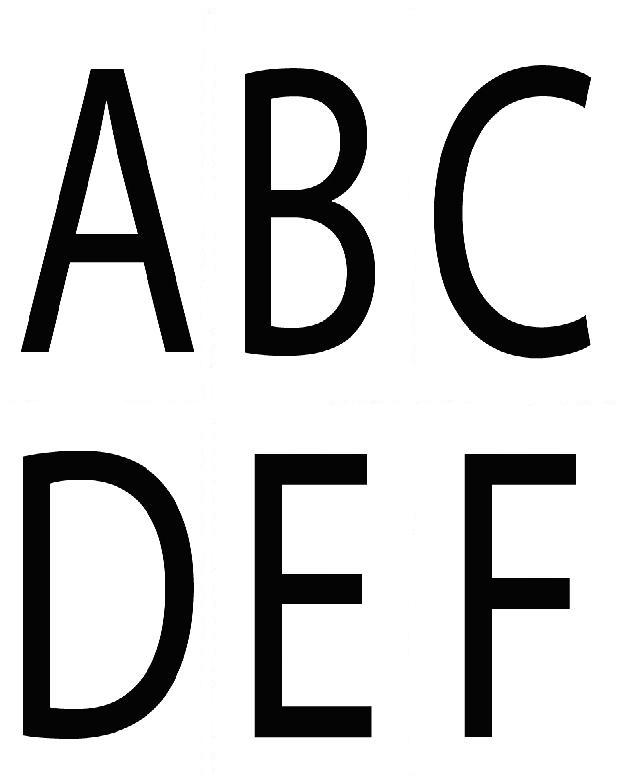
\includegraphics[width=0.7\textwidth]{abcdef.png}
\end{minipage}\vspace{3pt}

\noindent\begin{minipage}{0.75\textwidth}\parindent15pt
\begin{esercizio}
	\label{ese:8.25}
	Le due rette tracciate sono assi di simmetria del rettangolo in grigio a fianco e pertanto lo sono anche per l'immagine in esso contenuta. Vero o falso?
\end{esercizio}
\end{minipage}\hfil
\begin{minipage}{0.25\textwidth}
	\centering~~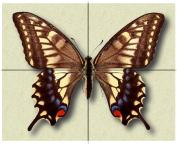
\includegraphics[width=0.75\textwidth]{butterfly.png}
\end{minipage}%\vspace{5pt}

\begin{esercizio}
\label{ese:8.26}
Perché la retta che congiunge i punti medi dei lati obliqui di un trapezio isoscele non è un suo asse di simmetria?
\end{esercizio}

\begin{esercizio}
\label{ese:8.27}
In $S_x$ (simmetria assiale rispetto all'asse $x$) il segmento $AB$ di estremi $A(3;2)$ e $B(3;-2)$
\begin{enumeratea}
\item è unito, luogo di punti uniti;
\item non ha punti fissi;
\item ha tutti i suoi punti uniti tranne $A$ e $B$;
\item ha un solo punto fisso;
\item ha solo $A$ e $B$ fissi.
\end{enumeratea}
\end{esercizio}

\begin{esercizio}
\label{ese:8.28}
Dimostrate che un qualunque segmento $MN$ di estremi $M(a;b)$ e $N(c;d)$ ha come corrispondente sia nella simmetria avente come asse l'asse $x$, sia nella simmetria avente come asse l'asse $y$, il segmento $M'N'$ tale che $MN\cong M'N'$.\vspace{5pt}

\noindent Ipotesi: $M(a;b)$, $N(c;d)$, $S_x:(M\rightarrow M') \wedge (N\rightarrow N')$\\
Tesi: $MN\cong M'N'$\vspace{3pt}\\
\emph{Dimostrazione.}\\
Determino $\overline{MN}=\ldots{}$ Trovo $M'(\ldots{};\ldots{})$ e $N'(\ldots{};\ldots{})$. Determino $\overline{M'N'}=\ldots{}$\\
Concludo: \ldots{}\vspace{5pt}

\noindent Ipotesi: $M(a;b)$, $N(c;d)$, $S_y:(M\rightarrow M') \wedge (N\rightarrow N')$\\
Tesi: $MN\cong M'N'$\vspace{3pt}\\
\emph{Dimostrazione.}\\
Determino $\overline{MN}=\ldots{}$ Trovo $M'(\ldots{};\ldots{})$ e $N'(\ldots{};\ldots{})$. Determino $\overline{M'N'}=\ldots{}$\\
Concludo: \ldots{}
\end{esercizio}

\begin{esercizio}
\label{ese:8.29} % 33
Il triangolo $ABC$ è isoscele; sapendo che $A(0;4)$, $B(-2;0)$ e che l'asse $x$ è il suo asse di simmetria, determinate il vertice $C$, il perimetro e l'area del triangolo.
\end{esercizio}

\begin{esercizio}
\label{ese:8.30} % 34
Il triangolo $ABC$ è isoscele; sapendo che $A(0;4)$, $B(-2;0)$ e che l'asse $y$ è il suo asse di simmetria, determinate il vertice $C$, il perimetro e l'area del triangolo.
\end{esercizio}

\noindent\begin{minipage}{0.45\textwidth}\parindent15pt
\begin{esercizio}
\label{ese:8.31} % 35
Considerate la funzione di proporzionalità quadratica $y=2x^2$. Rappresentatela nel riferimento cartesiano e segnate i suoi punti $A$, $B$ e $C$, rispettivamente di ascissa $x_A=1$, $x_B=-\frac{1}{2}$ e $x_C=\frac{1}{\sqrt{2}}$; trovate i corrispondenti $A'$, $B'$, $C'$ nella simmetria $S_y$ e verificate che appartengono alla funzione assegnata. Vi è un punto della curva rappresentata che risulta fisso in $S_y$? Inoltre, quale delle seguenti affermazioni ritenete corretta:
\begin{enumeratea}
\item la curva è fissa nella simmetria considerata;
\item la curva è unita nella simmetria considerata.
\end{enumeratea}
\end{esercizio}
\end{minipage}\hfil
\begin{minipage}{0.55\textwidth}
	\centering% (c) 2014 Daniele Masini - d.masini.it@gmail.com
\begin{tikzpicture}[scale=1,font=\small, x=5.9mm, y=5.9mm, smooth]
\usetikzlibrary{calc}

\begin{scope}

\begin{scope}[dotted,orange]
\draw[step=5.9mm] (-5.5,-5.5) grid (5.7,5.7);
\end{scope}

\begin{scope}[->]
\draw (-5.5,0) -- (5.7,0) node [below] {$x$};
\draw (0,-5.5) -- (0,5.7) node [left] {$y$};
\end{scope}

\foreach \x in {-5, -4, -3, -2, -1, 1, 2, 3, 4, 5}
\draw (\x,1.5pt) -- (\x,-1.5pt) node[below] {$\x$};

\foreach \y in {-5, -4, -3, -2, -1, 1, 2, 3, 4, 5}
\draw (1.5pt,\y) -- (-1.5pt,\y) node[left] {$\y$};

\node[below left] at (0,0) {O};
%\filldraw[fill=white, draw=black] (0,0) circle (2pt);

\end{scope}


\end{tikzpicture}

\end{minipage}\vspace{4pt}

\begin{esercizio}
\label{ese:8.32} % 38
I punti $A(-5;1)$, $B(-2;6)$, $C(3;6)$ e $D(0;1)$ sono vertici di un quadrilatero.
\begin{enumeratea}
\item Dimostrate che è un parallelogrammo.
\item Determinate perimetro e area;
\item Determinate la sua immagine $A'B'C'D'$ in $S_{y=3}$.
\end{enumeratea}
\`E vero che sia sul lato $AB$ che sul lato $CD$ esiste un punto fisso nella simmetria considerata? Tali punti su quali lati di $A'B'C'D'$ si trovano? Perché?
\end{esercizio}

\begin{esercizio}
\label{ese:8.33} % 40
Determinate l'immagine del quadrilatero $ABCD$ di vertici $A(0;0)$, $B(2;2)$, $C(5;3)$, $D(0;5)$ nella simmetria $S_{b1}$.
\end{esercizio}

\begin{esercizio}
\label{ese:8.34} % 41
Nella simmetria $S_{b1}$ la retta $y=-x$ è fissa o unita?
\end{esercizio}

\begin{esercizio}
\label{ese:8.35} % 42
Motivate la verità della seguente proposizione: <<nella simmetria $S_{b2}$ l'immagine dell'asse $x$ è l'asse $y$>>. Viene mantenuto l'orientamento dell'asse $x$?
Completate: $S_{b2}:(\text{asse }x)\rightarrow (\text{asse } \ldots{})$ e $(\text{asse }y)\rightarrow(\ldots\ldots{})$
Analogamente: $S_{b1}:(\text{asse }x)\rightarrow (\text{asse } \ldots{})$ e $(\text{asse }y)\rightarrow(\ldots\ldots{})$
\end{esercizio}

\begin{esercizio}
\label{ese:8.36} % 43
Dato il quadrilatero $ABCD$ di vertici $A(0;0)$, $B(3;1)$, $C(4;4)$ e $D(1;3)$ trovate il suo corrispondente in $S_{b1}$. Quale delle seguenti affermazioni ritenete corretta:
\begin{enumeratea}
\item il quadrilatero è fisso nella simmetria considerata;
\item il quadrilatero è unito nella simmetria considerata.
\end{enumeratea}
\end{esercizio}

\begin{esercizio}
\label{ese:8.37} % 44
Determinate il corrispondente del parallelogramma $ABCD$ di vertici $A(-5;1)$, $B(-2;6)$, $C(3;6)$, $D(0;1)$ in $S_{b1}$; perché $AA'$, $BB'$, $CC'$ e $DD'$ sono paralleli? Ricordando che il parallelogramma ha un centro di simmetria, determinate il centro di simmetria di $ABCD$ e verificate che in $S_{b1}$ esso ha come immagine il centro di simmetria di $A'B'C'D'$.
\end{esercizio}

\begin{esercizio}
\label{ese:8.38} % 45
Nel piano cartesiano sono assegnati i punti $A(0;3)$, $B(-2;0)$ e $C(-1;-3)$.
\begin{enumeratea}
\item Determinate i punti $A'$, $B'$ e $C'$ immagine in $S_{b2}$.
\item Calcolate l'area del quadrilatero $A'B'C'O$, essendo $O$ l'origine del riferimento.
\item Motivate la verità della proposizione: <<i segmenti $AB$ e $A'B'$ si incontrano in un punto $P$ della bisettrice del II\textsuperscript{o}-IV\textsuperscript{o} quadrante>>.
\item \`E vero che $AP'B$ è congruente a $PAB'$?
\end{enumeratea}
\end{esercizio}

\begin{esercizio}
\label{ese:8.39} % 46
Sono assegnate le simmetrie
\[S_1:\begin{cases}x'=-x\\y'=-y\end{cases};\quad S_2:\begin{cases}x'=y\\y'=x\end{cases};\quad
S_3:\begin{cases}x'=2-x\\y'=y\end{cases};\quad S_4:\begin{cases}x'=-x-1\\y'=3-y\end{cases}\]
Usando qualche punto scelto arbitrariamente riconosci ciascuna di esse e completa la tabella sottostante:
\begin{center}
\begin{tabular}{cccc}
\toprule
Simmetria & Tipo & Centro (coordinate) & Asse (equazione)\\
\midrule
$S_1$ & \ldots\ldots\ldots{} & \ldots\ldots{} & \ldots\ldots\ldots{} \\
$S_2$ & \ldots\ldots\ldots{} & \ldots\ldots{} & \ldots\ldots\ldots{} \\
$S_3$ & \ldots\ldots\ldots{} & \ldots\ldots{} & \ldots\ldots\ldots{} \\
$S_4$ & \ldots\ldots\ldots{} & \ldots\ldots{} & \ldots\ldots\ldots{} \\
\bottomrule
\end{tabular}
\end{center}
\end{esercizio}

\begin{esercizio}
\label{ese:8.40} % 47
Quale tra le seguenti caratteristiche è invariante in una simmetria assiale?
\begin{enumeratea}
\item la posizione della figura;
\item la direzione della retta;
\item il parallelismo;
\item l'orientamento dei punti;
\item dipende dall'asse di simmetria.
\end{enumeratea}
\end{esercizio}

\begin{esercizio}
\label{ese:8.41} % 48
I segmenti $AB$ e $A'B'$ si corrispondono nella simmetria di asse $r$; sapendo che $ABB'A'$ è un rettangolo, quale proposizione è vera?
\begin{enumeratea}
\item $AB$ è perpendicolare ad $r$;
\item $AB$ è parallelo ad $r$;
\item $AB$ appartiene ad $r$;
\item $AB$ è obliquo rispetto ad $r$ e $AB\cap r=H$.
\end{enumeratea}
\end{esercizio}

\begin{esercizio}
\label{ese:8.42} % 49
\`E assegnato il punto $P\left(-\sqrt{3};\dfrac{\sqrt{2}-1}{2}\right)$. Determinate il suo corrispondente nelle simmetrie indicate e completate:
\begin{center}
\begin{tabular}{ccc}
$S_{b2}:P\rightarrow P'(\ldots{};\ldots{})$ & $S_{x=-\frac{1}{2}}:P\rightarrow P'(\ldots{};\ldots{})$ & $S_{O}:P\rightarrow P'(\ldots{};\ldots{})$\\
$S_{x}:P\rightarrow P'(\ldots{};\ldots{})$ & $S_{y=2}:P\rightarrow P'(\ldots{};\ldots{})$ & $S_{C(1;1)}:P\rightarrow P'(\ldots{};\ldots{})$\\
\end{tabular}
\end{center}
\end{esercizio}

\begin{esercizio}
\label{ese:8.43} % 50
Un segmento unito in $S_{b2}$ è
\begin{enumeratea}
\item un segmento perpendicolare alla bisettrice del I\textsuperscript{o}-III\textsuperscript{o} quadrante;
\item un segmento perpendicolare alla bisettrice del II\textsuperscript{o}-IV\textsuperscript{o} quadrante nel suo punto medio;
\item un segmento parallelo alla bisettrice del I\textsuperscript{o}-III\textsuperscript{o} quadrante;
\item un segmento perpendicolare alla bisettrice del II\textsuperscript{o}-IV\textsuperscript{o} quadrante;
\item un segmento avente il suo punto medio appartenente alla bisettrice del II\textsuperscript{o}-IV\textsuperscript{o} quadrante.
\end{enumeratea}
\end{esercizio}

\noindent\begin{minipage}{0.75\textwidth}\parindent15pt
\begin{esercizio}
\label{ese:8.44} % 51
Nel piano sono assegnati i tre punti $A$, $B$ e $A'$ dei quali il punto $A'$ è immagine di $A$ in una traslazione. Dopo aver determinato il vettore della traslazione costruite l'immagine del triangolo $ABA'$.
\end{esercizio}
\end{minipage}\hfil
\begin{minipage}{0.25\textwidth}
	\centering~~% (c) 2014 Daniele Masini - d.masini.it@gmail.com
\begin{tikzpicture}[scale=1,font=\small]
\usetikzlibrary{calc}

\begin{scope}
\draw[fill] (0,0) circle (1pt) node[above right] {$B$};
\draw[fill] (0,1.2) circle (1pt) node[above right] {$A$};
\draw[fill] (1.8,0) circle (1pt) node[above right] {$A'$};
\end{scope}

\end{tikzpicture}

\end{minipage}\vspace{8pt}

\begin{esercizio}
\label{ese:8.45} % 52
Determinate l'immagine del parallelogrammo $ABCD$ nella traslazione di vettore $\vec{v} \equiv \overrightarrow{AC}$.
\end{esercizio}

\noindent\begin{minipage}{0.75\textwidth}\parindent15pt
\begin{esercizio}
\label{ese:8.46} % 53
Dati due punti distinti $A$ e $B$ e il vettore $\overrightarrow{CD}$ della figura a fianco, detti $A'$ e $B'$ i punti immagine di $A$ e $B$ nella traslazione di vettore $\overrightarrow{CD}$, rispondete alle domande:
\begin{enumeratea}
\item Di che natura è il quadrilatero $ABB'A'$?
\item Può succedere che il quadrilatero in questione sia un rettangolo? E un rombo?
\item Cosa succede se $AB$ è parallelo al vettore $\overrightarrow{CD}$?
\end{enumeratea}
\end{esercizio}
\end{minipage}\hfil
\begin{minipage}{0.25\textwidth}
	\centering~~% (c) 2014 Daniele Masini - d.masini.it@gmail.com
\begin{tikzpicture}[scale=1,font=\small]
\usetikzlibrary{calc}

\begin{scope}
\draw[fill] (0,0) coordinate (c) circle (1pt) node[above right] {$C$};
\draw[fill] (1.7,0) coordinate (d) circle (1pt) node[above right] {$D$};
\draw[thick, blue, ->] (c) -- (d);
\draw[fill] (-0.4,-0.8) coordinate (a) circle (1pt) node[above right] {$A$};
\draw[fill] (0.7,-1.7) coordinate (b) circle (1pt) node[above right] {$B$};
\end{scope}

\end{tikzpicture}

\end{minipage}\vspace{8pt}

\begin{esercizio}
\label{ese:8.47} % 54
Come dobbiamo assegnare due segmenti $AB$ e $A'B'$ affinché siano corrispondenti in una traslazione? \`E unica la traslazione che associa ad $AB$ il segmento $A'B'$?
\end{esercizio}

\begin{esercizio}
\label{ese:8.48} % 58
Nel riferimento cartesiano è assegnato il punto $P(-4;2)$. Determinate il punto $P'$ immagine nella traslazione $T(3;-1):\begin{cases}x'=x+3\\y'=y+(-1)\end{cases}$.\\
Strategia risolutiva:
\begin{enumerate*}
\item individuate il vettore $\vec{w}$ della traslazione: $\vec{w}(\ldots{};\ldots{})$;
\item tracciate il vettore nel riferimento cartesiano;
\item determinate le coordinate di $P'$: $P'(\ldots{};\ldots{})$.
\end{enumerate*}
Completate: $\overrightarrow{PP'}$ è \ldots\ldots\ldots{} a $\vec{w}$; questo significa che i due vettori hanno \ldots\ldots\ldots{} direzione (cioè sono \ldots\ldots\ldots{}), stesso \ldots\ldots\ldots{} e \ldots\ldots\ldots{} intensità.
\end{esercizio}

\begin{esercizio}
\label{ese:8.49} % 59
Nel riferimento cartesiano, dopo aver fissato il punto $P(-4;2)$ siano dati i punti $Q(\ldots{};\ldots{})$ e $Q'(\ldots{};\ldots{})$ immagine nella traslazione $T(3;-1)$. Dimostrate con le conoscenze di geometria sintetica che $PP'Q'Q$ è un parallelogramma.\vspace{5pt}\\
\noindent Ipotesi: $PP'\cong QQ'$, $PP'\ldots{}QQ'$\\
Tesi: \ldots\ldots\ldots{}\vspace{3pt}\\
\emph{Dimostrazione. \ldots\ldots{}}
\end{esercizio}

\begin{esercizio}
\label{ese:8.50} % 60
Sappiamo che l'equazione di una traslazione è $T(a;b):\begin{cases}x'=x+a\\y'=y+b\end{cases}$. Assegnate le coordinate $(x;y)$ di un punto $P$ e $(x';y')$ della sua immagine $P'$, le componenti del vettore della traslazione sono date da:
\begin{multicols}{2}
\begin{enumeratea}
\item $a=x'+x$\quad e\quad $b=y'+y$;
\item $a=x-x'$\quad e\quad $b=y-y'$;
\item $a=x'-x$\quad e\quad $b=y'-y$;
\item $a=x'+x$\quad e\quad $b=y'-y$;
\item $a=\dfrac{x'}{x}$\quad e\quad $b=\dfrac{y'}{y}$.
\end{enumeratea}
\end{multicols}
\end{esercizio}


\begin{esercizio}
\label{ese:8.51} % 61
Dopo aver determinato l'equazione della traslazione in cui $A'(0;-2)$ è l'immagine di $A(3;2)$, determinate il perimetro del triangolo $AO'A'$ essendo $O'$ il corrispondente di $O(0;0)$ nella traslazione trovata.
\end{esercizio}

\begin{esercizio}
\label{ese:8.52} % 62
Verificate che il punto medio $M$ del segmento $PQ$ di estremi $P(-1;4)$ e $Q(5;0)$ ha come immagine in $T(3;-1)$ il punto medio $M'$ del segmento $P'Q'$.
\end{esercizio}

\begin{esercizio}
\label{ese:8.53} % 63
Applica la traslazione di equazione $\begin{cases}x'=x+2\\y'=y-1\end{cases}$ al segmento di estremi $A(-2;4)$ e $B(3;3)$. 
\end{esercizio}

\begin{esercizio}
\label{ese:8.54} % 64
Dati $A(1;0)$ e $B(0;2)$, determina $C$ e $D$ in modo che $ABCD$ sia un quadrato.
\end{esercizio}

\begin{esercizio}
\label{ese:8.55} % 65
Determinate l'immagine del triangolo di vertici $A(0;2)$, $B(-3;2)$ e $C(0;5)$ nella traslazione $T(4;1)$. Calcolatene quindi perimetro e area.
\end{esercizio}

\begin{esercizio}
\label{ese:8.56} % 66
Determinate l'equazione della traslazione di vettore $\vec{s}=\vec{u}+\vec{v}$ assegnati dalla figura~\ref{fig:ese8.56}. Determinate inoltre l'immagine del poligono di vertici $H(-1;1)$, $K(0;-2)$, $L(3;0)$ ed $F(1;2)$.
\end{esercizio}

\begin{figure}[!htb]
	\centering% (c) 2014 Daniele Masini - d.masini.it@gmail.com
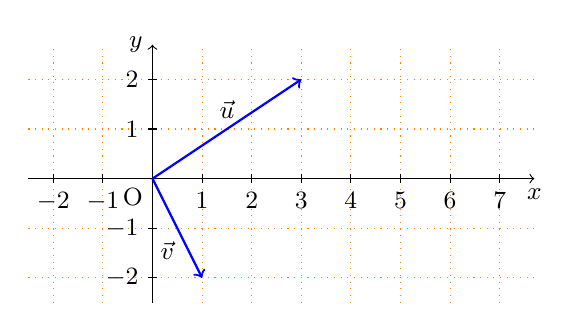
\begin{tikzpicture}[scale=1,font=\small, x=6.3mm, y=6.3mm, smooth]
\usetikzlibrary{calc}

\begin{scope}

\begin{scope}[dotted,orange]
\draw[step=6.3mm] (-2.5,-2.5) grid (7.7,2.7);
\end{scope}

\begin{scope}[->]
\draw (-2.5,0) -- (7.7,0) node [below] {$x$};
\draw (0,-2.5) -- (0,2.7) node [left] {$y$};
\end{scope}

\foreach \x in {-2, -1, 1, 2, 3, 4, 5, 6, 7}
\draw (\x,1.5pt) -- (\x,-1.5pt) node[below] {$\x$};

\foreach \y in {-2, -1, 1, 2}
\draw (1.5pt,\y) -- (-1.5pt,\y) node[left] {$\y$};

\node[below left] at (0,0) {O};
%\filldraw[fill=white, draw=black] (0,0) circle (2pt);

\draw[thick, blue, ->] (0,0) -- node [black, above] {$\vec{u}$} (3,2);
\draw[thick, blue, ->] (0,0) -- node [black, shift={(-0.2,-0.45)}] {$\vec{v}$} (1,-2);

\end{scope}


\end{tikzpicture}

	\caption{Esercizio~\ref{ese:8.56}}\label{fig:ese8.56}
\end{figure}\vspace{8pt}

\begin{esercizio}
\label{ese:8.57} % 67
Un vettore $\vec{v}$ ha modulo unitario, è applicato nell'origine $O$ e forma con l'asse delle ascisse un angolo di $30\grado$. Determinate le sue componenti e scrivete l'equazione della traslazione da esso caratterizzata.
\end{esercizio}

\noindent\begin{minipage}{0.7\textwidth}\parindent15pt
\begin{esercizio}
\label{ese:8.58} % 68
Prendete in considerazione l'angolo $\epsilon$ di vertice $T$ della figura a fianco. Sia $O$ il centro di rotazione e $F$ un punto del piano di cui si vuole determinare l'immagine. Costruite $F'$ seguendo i passi illustrati immediatamente dopo la definizione~\ref{def:rotaz} a pagina~\pageref{def:rotaz}.
\end{esercizio}
\end{minipage}\hfil
\begin{minipage}{0.3\textwidth}
	\centering~~% Copyright (c) 2015 Daniele Masini - d.masini.it@gmail.com

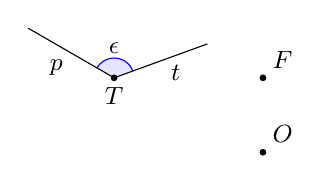
\begin{tikzpicture}[scale=1,font=\small, x=6.3mm, y=6.3mm, smooth]
\usetikzlibrary{calc}

\begin{scope}
\coordinate (t) at (0,0);
\coordinate (f) at (3,0);
\coordinate (o) at (3,-1.5);
\path (t) -- +(20:2) coordinate (t1);
\path (t) -- +(150:2) coordinate (t2);

\begin{scope}
\clip (t1) -- (t) -- (t2) -- cycle;
\draw[blue, fill=blue!10] (t) circle (0.4) node [black, shift={(90:0.6)}] {$\epsilon$};
\end{scope}

\draw (t) -- node[shift={(0.3,-0.25)}] {$t$} (t1);
\draw (t) -- node[shift={(-0.3,-0.3)}] {$p$} (t2);

\draw[fill] (t) circle (1pt) node [below] {$T$};
\draw[fill] (f) circle (1pt) node [above right] {$F$};
\draw[fill] (o) circle (1pt) node [above right] {$O$};

\end{scope}


\end{tikzpicture}

\end{minipage}\vspace{8pt}

\begin{esercizio}
\label{ese:8.59} % 69
Costruite l'immagine del quadrato $ABCD$ nella rotazione di $+90\grado$ avente come centro di simmetria il vertice $B$.
Fissate i punti medi $M$ ed $N$ rispettivamente di $AB$ e di $CD$; dove si trovano le rispettive immagini?
\end{esercizio}

\begin{esercizio}
\label{ese:8.60} % 70
\`E vero che il quadrato è unito nella rotazione avente come centro il punto di incontro delle diagonali e come ampiezza $90\grado$?
\end{esercizio}

\begin{esercizio}
\label{ese:8.61} % 71
L'ortocentro di un triangolo equilatero è il centro di una rotazione in cui il triangolo è unito. Determinate l'angolo di rotazione.
\end{esercizio}

\begin{esercizio}
\label{ese:8.62} % 72
Costruite l'immagine $A'B'C'$ del triangolo equilatero $ABC$ nella rotazione di centro $B$ e ampiezza $-120\grado$. Dimostrate che $C$, $B$ ed $A'$ sono allineati e che $ABC'$ è un triangolo equilatero congruente a quello dato.
\end{esercizio}

\noindent\begin{minipage}{0.75\textwidth}\parindent15pt
\begin{esercizio}
\label{ese:8.63} % 73
Nel piano è assegnato il punto $C$ e il vettore $\vec{v}$ (figura a lato); costruite l'immagine del punto $P$ nell'isometria $T_{\vec{v}} \circ S_{C}$ e anche l'immagine dello stesso punto $P$ nell'isometria $S_{C} \circ T_{\vec{v}}$. Determinate l'equazione di $\Phi_1 = T_{\vec{v}} \circ S_{C}$ e di $\Phi_2 = S_{C} \circ T_{\vec{v}}$.
\end{esercizio}
\end{minipage}\hfil
\begin{minipage}{0.25\textwidth}
	\centering~~% (c) 2014 Daniele Masini - d.masini.it@gmail.com
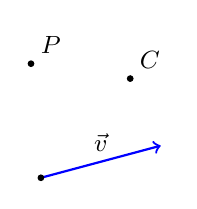
\begin{tikzpicture}[scale=1,font=\small, x=6.3mm, y=6.3mm, smooth]
\usetikzlibrary{calc}

\begin{scope}
\coordinate (v) at (0,0);
\coordinate (c) at (1.8,2);
\coordinate (p) at (-.2,2.3);
\path (v) -- +(15:2.5) coordinate (v1);

\draw[blue, thick, ->] (v) -- node [black, above] {$\vec{v}$} (v1);

\draw[fill] (v) circle (1pt);
\draw[fill] (c) circle (1pt) node [above right] {$C$};
\draw[fill] (p) circle (1pt) node [above right] {$P$};

\end{scope}


\end{tikzpicture}

\end{minipage}\vspace{8pt}

\begin{esercizio}
\label{ese:8.64} % 74
Il centro della simmetria è il punto $C(-1;-2)$, il vettore della traslazione è $\vec{v}(3;-2)$ e il punto di cui vogliamo determinare l'immagine è scelto da voi arbitrariamente. 
\end{esercizio}

\begin{esercizio}
\label{ese:8.65} % 75
Sono assegnati il punto $C(-4;3)$, la retta $x=1$ e il punto $P(0;5)$. Determinate l'immagine $P''$ di $P$ nell'isometria $\Delta=S_{C}\circ S_{x=1}$ e l'immagine $P^*$ di $P$ nell'isometria $\Delta=S_{x=1}\circ S_{C}$. \`E vero che $P''$ e $P^*$ si corrispondono nella simmetria $S_y$? Determinate l'area del triangolo $PP''P^*$.
\end{esercizio}

\begin{esercizio}
\label{ese:8.66} % 76
\`E assegnato un punto $O$; determinate l'immagine $P'$ di un punto $P$ nella rotazione di centro $O$ e angolo di $60\grado$ e l'immagine $P''$ di $P'$ nella simmetria avente come asse la retta $PO$.
\begin{enumeratea}
\item Completate: $P \overset{\ldots{}}\longrightarrow P'$. 
\item Dimostrate che $P$, $P'$ e $P''$ appartengono alla circonferenza di centro $O$ e raggio $OP$.
\item Individuate le caratteristiche del quadrilatero $PP''OP'$.
\item Determinatene l'area, supponendo $\overline{OP}=2$~m.
\end{enumeratea}
\end{esercizio}

\begin{esercizio}
\label{ese:8.67} % 80
$ABC$ è un triangolo equilatero e $O$ è il centro della sua circonferenza circoscritta. Dimostrate che il triangolo è unito nella rotazione di centro $O$ e angolo $\alpha=120\grado$. Analogamente il quadrato $ABCD$ è unito nella rotazione di centro $H$, punto di incontro delle sue diagonali, di angolo $\alpha=90\grado$.
\end{esercizio}

\begin{esercizio}
\label{ese:8.68} % 81
Giustificate la verità della proposizione: <<La simmetria centrale di centro $K$ è una rotazione di $180\grado$>>.
\end{esercizio}

\begin{esercizio}
\label{ese:8.69} % 82
Nel piano dotato di riferimento cartesiano è tracciata la bisettrice del I\textsuperscript{o} e III\textsuperscript{o} quadrante e la retta $y=1$. Completate le osservazioni seguenti:
\begin{enumeratea}
\item il punto di intersezione $K$ ha coordinate $K(\ldots{};\ldots{})$;
\item l'angolo delle due rette è di $\ldots{}\grado$.
\end{enumeratea}
\end{esercizio}

\begin{esercizio}
\label{ese:8.70} % 83
Scrivete l'equazione della simmetria avente come asse la bisettrice: $S_{b1}\begin{cases}x'=\ldots{}\\y'=\ldots{}\end{cases}$ e l'equazione della simmetria di asse la retta $y=1$: $S_{y=1}\begin{cases}x'=\ldots{}\\y'=\ldots{}\end{cases}$.
\end{esercizio}

\begin{esercizio}
\label{ese:8.71} % 84
Determinate le coordinate del punto $P''$ immagine di $P$, arbitrariamente scelto, in $\Omega = S_{b1} \circ S_{y=1}$ e scrivete l'equazione di $\Omega$.
Concludete: $\Omega$ è la rotazione di centro \ldots{} e angolo \ldots{} (ricordate il segno dell'angolo di rotazione).
\end{esercizio}

\begin{esercizio}
\label{ese:8.72} % 85
Determinate le coordinate del punto $P^*$ immagine di $P$, arbitrariamente scelto, in $\Omega^*=S_{y=1} \circ S_{b1}$ e scrivete l'equazione di $\Omega^*$.
Concludete: $\Omega^*$ è la rotazione di centro \ldots{} e angolo \ldots{} (ricordate il segno dell'angolo di rotazione).
\end{esercizio}

\begin{esercizio}
\label{ese:8.73} % 86
Determinate l'equazione della isometria $J=S_{b1} \circ S_{x=4}$ e stabilite se esiste qualche elemento unito. Come cambia l'equazione dell'isometria $J^*=S_{x=4} \circ S_{b1}$ rispetto alla precedente? Sia $J$ che $J^*$ sono rotazioni: determinate centro e angolo (con segno) di ognuna di esse. A questo scopo potete utilizzare il punto $P(2;4)$ o un punto arbitrariamente scelto.
\end{esercizio}

\noindent\begin{minipage}{0.7\textwidth}\parindent15pt
\begin{esercizio}
\label{ese:8.74} % 87
Determinate l'immagine del punto $A$ nell'isometria $\Delta=S_b \circ S_a$ essendo $a$ e $b$ le rette parallele segnate nella figura a fianco e $A$ il punto dato. Dimostrate che $\overline{AA''}=2\cdot d$ essendo $d$ la distanza tra le rette $a$ e $b$.
Fissate arbitrariamente un altro punto $B$ non appartenente ad alcuna delle rette date e determinate la sua immagine $B''$ nell'isometria $\Delta$.
\`E vero che $\overline{AA''}=\overline{BB''}$ e $\overline{AA''} \parallel \overline{BB''}$? Potete concludere che l'isometria $\Delta$ è la traslazione di vettore $\overrightarrow{AA''}$?
\end{esercizio}
\end{minipage}\hfil
\begin{minipage}{0.3\textwidth}
	\centering~~% Copyright (c) 2015 Daniele Masini - d.masini.it@gmail.com

\begin{tikzpicture}[scale=1,font=\small]
\usetikzlibrary{calc}

\begin{scope}
\coordinate (a) at (0,0);

\draw[blue, thick] (-1.5,-0.5) -- (1.5,-0.5) node [black, above] {$a$};
\draw[blue, thick] (-1.5,-1.5) -- (1.5,-1.5) node [black, above] {$b$};

\draw[fill] (a) circle (1pt) node [above right] {$A$};

\end{scope}


\end{tikzpicture}


\end{minipage}\vspace{8pt}

\begin{esercizio}
\label{ese:8.75} % 88
Facendo riferimento all'esercizio~\ref{ese:8.74}, verificate che la traslazione $\Delta_1 = S_a \circ S_b$ è caratterizzata da un vettore avente modulo e direzione uguali al vettore $\overrightarrow{AA''}$ ma verso opposto.
\end{esercizio}

\begin{esercizio}
\label{ese:8.76} % 89
Nel riferimento cartesiano ortogonale sono assegnati i punti $A(1;5)$, $B(2;1)$ e $C(-1;3)$. Determinate i punti $A''$, $B''$ e $C''$ immagine rispettivamente di $A$, $B$ e $C$ nella traslazione $T=S_{x=-2} \circ S_{x=1}$. Scrivete l'equazione della traslazione, individuate il vettore che la definisce calcolandone modulo e direzione.
\end{esercizio}

\begin{esercizio}
\label{ese:8.77} % 90
Determinate i vettori $\vec{u}$ e $\vec{v}$ delle traslazioni $T_{\vec{u}}\begin{cases}x'=x+1\\y'=y-2\end{cases}$ e $T_{\vec{v}}\begin{cases}x'=x-3\\y'=y-1\end{cases}$ e il vettore $\vec{s} = \vec{u} + \vec{v}$. Verificate che $T_{\vec{s}} = T_{\vec{u}} \circ T_{\vec{v}}$.
Cosa otteniamo dalla composizione $T_{\vec{u}} \circ T_{\vec{v}}$? Sapresti darne la motivazione?
Concludete: componendo due traslazioni si ottiene \ldots\ldots{}
\end{esercizio}

\begin{esercizio}
\label{ese:8.78} % 91
Nel riferimento cartesiano ortogonale $Oxy$ è assegnato il punto $O_1(2;1)$; scrivete l'equazione della simmetria centrale di centro $O$ $S_O\begin{cases}x'=\ldots{}\\y'=\ldots{}\end{cases}$  e l'equazione della simmetria centrale di centro $O_1$ $S_{O_1}\begin{cases}x'=\ldots{}\\y'=\ldots{}\end{cases}$. Determinate l'immagine $P''$ del punto $P(1;2)$ nell'isometria $\Sigma=S_O \circ S_{O_1}$ di cui avrete scritto l'equazione e determinate $\overline{PP''}$. Determinate $Q''$ immagine di $Q\left(\frac{1}{2};-1\right)$ nell'isometria $\Sigma$ e determinate $\overline{QQ''}$. Potete affermare che $\overrightarrow{PP''} \equiv \overrightarrow{QQ''}$? Verificate che $\overrightarrow{PP''} \equiv \overrightarrow{QQ''} \equiv 2\cdot \overrightarrow{O_1O}$.
\`E vero che $\Sigma=S_O \circ S_{O_1}$ e $\Sigma_1=S_{O_1} \circ S_{O}$ sono la stessa isometria?
\end{esercizio}

\begin{esercizio}
\label{ese:8.79} % 93
Dimostrate che la composizione di due simmetrie centrali è una traslazione caratterizzata dal vettore parallelo alla retta passante per i due centri e modulo uguale al doppio della loro distanza.
\end{esercizio}

\begin{esercizio}
\label{ese:8.80} % 94
Si consideri la composizione di due simmetrie assiali con assi paralleli $S_b\begin{cases}x'=2b-x\\y'=y\end{cases}$ e $S_a\begin{cases}x'=a-x\\y'=y\end{cases}$.
Componendo le due simmetrie si ha $S_b\begin{cases}x'=2b-2a+x\\y'=y\end{cases}$ che è \ldots\ldots{}
Se $a=b$ le due simmetrie sono \ldots\ldots{} la loro composizione è \ldots\dots{}
\end{esercizio}

\begin{esercizio}
\label{ese:8.81} % 95
Si consideri la composizione di due simmetrie assiali con assi perpendicolari.
Una simmetria con asse parallelo all'asse $y$ ha equazione $S_a\begin{cases}x'=2a-x\\y'=y\end{cases}$ e asse $x = a$.
Mentre una simmetria con asse parallelo all'asse $x$ ha equazione $S_b\begin{cases}x'=x\\y'=2b-y\end{cases}$ e asse $y = b$.
Componendo le due simmetrie otteniamo \ldots\ldots{}
\end{esercizio}

\begin{esercizio}
\label{ese:8.82} % 96
Verificate che:
\begin{enumeratea}
\item l'inversa della traslazione di vettore $\vec{v}(a;b)$ è la traslazione di vettore $-\vec{v}$;
\item l'inversa di una rotazione di centro $O$ e angolo $\alpha$ è la rotazione di centro $O$ e angolo $-\alpha$.
\end{enumeratea}
\end{esercizio}

\begin{esercizio}
\label{ese:8.83} % 97
Verificate che le simmetrie (centrale e assiale) hanno se stesse come isometria inversa, ossia $(S_K)^{-1}=S_K$ e $(S_r)^{-1}=S_r$.
\end{esercizio}

\begin{esercizio}
\label{ese:8.84} % 98
La proposizione <<la simmetria centrale è la composizione di due simmetrie assiali>> è:
\begin{enumeratea}
\item sempre vera;
\item vera se i due assi sono incidenti;
\item mai vera;
\item vera se i due assi sono perpendicolari;
\item vera se i due assi sono paralleli.
\end{enumeratea}
\end{esercizio}

\begin{esercizio}
\label{ese:8.85} % 99
Completa la proposizione: <<la simmetria centrale di centro $C\left(-\frac{5}{3};\sqrt{3}\right)$ può essere ottenuta come composizione delle due simmetrie assiali di assi le rette \ldots\ldots{} e \ldots\ldots{} e la sua equazione è \ldots\ldots\ldots{}
\end{esercizio}

\begin{esercizio}
\label{ese:8.86} % 100
Stabilite il valore di verità delle proposizioni:
%Componendo due isometrie si ottiene una isometria
\begin{enumeratea}
\item Componendo due simmetrie assiali si ottiene una simmetria assiale\hfill\boxV\quad\boxF
\item Componendo due traslazioni si ottiene una traslazione\hfill\boxV\quad\boxF
\item Componendo due simmetrie centrali si ottiene una simmetria centrale\hfill\boxV\quad\boxF
\item Componendo due simmetrie assiali di assi incidenti si ottiene una rotazione\hfill\boxV\quad\boxF
\item Componendo due rotazioni si ottiene una rotazione\hfill\boxV\quad\boxF
\item L'identità si ottiene componendo una isometria con sé stessa\hfill\boxV\quad\boxF
\item L'inversa di una traslazione è la stessa traslazione\hfill\boxV\quad\boxF
\item Componendo una simmetria centrale con una rotazione si ottiene l'identità\hfill\boxV\quad\boxF
\item Componendo una simmetria centrale di centro $H$ con la simmetria assiale avente come asse una retta passante per $H$ si ottiene sempre l'identità\hfill\boxV\quad\boxF
\end{enumeratea}
\end{esercizio}

\begin{esercizio}
\label{ese:8.87} % 101
L'equazione $\begin{cases}x'=4-x\\y'=y\end{cases}$ descrive: 
\begin{enumeratea}
\item la simmetria assiale di asse $y$;
\item la simmetria assiale di asse la retta $x=4$;
\item la traslazione di vettore $\vec{v}(4;0)$;
\item la simmetria assiale di asse $x=2$;
\item la simmetria centrale di centro $C(4;0)$.
\end{enumeratea}
\end{esercizio}

\begin{esercizio}
\label{ese:8.88} % 102
La trasformazione $\Sigma \begin{cases}x'=-y+2\\y'=2x\end{cases}$ è un'isometria?
\end{esercizio}

\begin{esercizio}
\label{ese:8.89} % 103
Il segmento di estremi $A(3;4)$ e $B(3;-2)$ ha come simmetrico il segmento di estremi $A'(3;2)$ e $B'(5;2)$; è stata eseguita:
\begin{enumeratea}
\item la simmetria assiale di asse la retta $x=4$;
\item la simmetria $S_{b2}$;
\item la simmetria $S_{b1}$;
\item la simmetria assiale di asse la retta $x=3$;
\item la simmetria $S_{y=3}$.
\end{enumeratea}
\end{esercizio}

\begin{esercizio}
\label{ese:8.90} % 104
Attribuisci il valore di verità alle seguenti proposizioni:
\begin{enumeratea}
\item In una isometria vi è almeno un elemento unito\hfill\boxV\quad\boxF
\item Nella simmetria centrale vi sono infinite rette unite, ma solamente un punto unito\tab\tab\hfill\boxV\quad\boxF
\item In ogni triangolo vi è almeno un asse di simmetria\hfill\boxV\quad\boxF
\item Qualche quadrilatero ha un centro di simmetria\hfill\boxV\quad\boxF
\item Il triangolo equilatero ha un centro di simmetria\hfill\boxV\quad\boxF
\item Il rombo è l'unico quadrilatero avente due assi di simmetria\hfill\boxV\quad\boxF
\item Tutte le rette aventi la stessa direzione del vettore della traslazione sono rette unite\tab\tab\hfill\boxV\quad\boxF
\item Solo la simmetria assiale è una isometria invertente\hfill\boxV\quad\boxF
\item Rette parallele hanno come immagine in una isometria rette parallele\hfill\boxV\quad\boxF
\item In una isometria una retta è sempre parallela alla sua immagine\hfill\boxV\quad\boxF
\end{enumeratea}
\end{esercizio}

\begin{esercizio}
\label{ese:8.91} % 105
Il quadrilatero di vertici $A(5;0)$, $B(9;0)$, $C(12;4)$ e $D(7;3)$ nella simmetria $S_x$ ha fisso il lato $AB$. Spiegate come sia possibile questo fatto.
\end{esercizio}

\begin{esercizio}
\label{ese:8.92} % 106
Dimostrate che la bisettrice di un angolo è il suo asse di simmetria.
\end{esercizio}

\begin{esercizio}
\label{ese:8.93} % 107
Il rettangolo $ABCD$ con $AB<BC$ ha come immagine il rettangolo $A'B'C'D'$ nella simmetria avente come asse la retta $AC$. Potete affermare che $AB'DCD'B$ è un esagono regolare?
\end{esercizio}

\noindent\begin{minipage}{0.75\textwidth}\parindent15pt
\begin{esercizio}
\label{ese:8.94} % 108
I due segmenti della figura a fianco possono essere corrispondenti in una simmetria centrale? 
\end{esercizio}
\end{minipage}\hfil
\begin{minipage}{0.25\textwidth}
	\centering~~% Copyright (c) 2015 Daniele Masini - d.masini.it@gmail.com

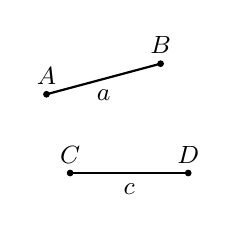
\begin{tikzpicture}[scale=1,font=\small]
\usetikzlibrary{calc}

\begin{scope}
\coordinate (a) at (0,0);
\path (a) -- +(15:1.5) coordinate (b);
\coordinate (c) at (0.3,-1);
\path (c) -- +(0:1.5) coordinate (d);

\draw[thick] (a) -- node [below] {$a$} (b);
\draw[thick] (c) -- node [below] {$c$} (d);

\draw[fill] (a) circle (1pt) node [above] {$A$};
\draw[fill] (b) circle (1pt) node [above] {$B$};
\draw[fill] (c) circle (1pt) node [above] {$C$};
\draw[fill] (d) circle (1pt) node [above] {$D$};

\end{scope}


\end{tikzpicture}


\end{minipage}\vspace{8pt}

\noindent\begin{minipage}{0.65\textwidth}\parindent15pt
\begin{esercizio}
\label{ese:8.95} % 109
Nella figura a fianco abbiamo disegnato il quadrato $ABCD$ e il punto $A'$ corrispondente di $A$ in una isometria. Stabilite quale isometria è completamente fissata con questi elementi (simmetria assiale, traslazione, simmetria centrale) e determinate in essa l'immagine del quadrato. 
\end{esercizio}
\end{minipage}\hfil
\begin{minipage}{0.35\textwidth}
	\centering~~% (c) 2014 Daniele Masini - d.masini.it@gmail.com
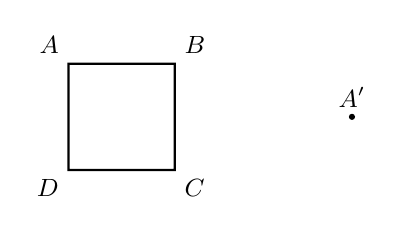
\begin{tikzpicture}[scale=0.9,font=\small]
\usetikzlibrary{calc}

\begin{scope}
\coordinate (a) at (0,0);
\path (a) -- +(0:1.5) coordinate (b);
\path (b) -- +(270:1.5) coordinate (c);
\path (c) -- +(180:1.5) coordinate (d);
\coordinate (a1) at (4,-0.75);

\draw[thick] (a) -- (b) -- (c) -- (d) -- cycle;

\node[above left] at (a) {$A$};
\node[above right] at (b) {$B$};
\node[below right] at (c) {$C$};
\node[below left] at (d) {$D$};

\draw[fill] (a1) circle (1pt) node[above] {$A'$};

\end{scope}


\end{tikzpicture}


\end{minipage}\vspace{8pt}

\begin{esercizio}
\label{ese:8.96} % 110
Costruite l'immagine di un triangolo rettangolo $ABC$ (non isoscele) di ipotenusa $BC$
\begin{enumeratea}
\item in ciascuna delle simmetrie $S_A$, $S_B$ e $S_C$;
\item nella simmetria $S_M$ essendo $M$ il punto medio dell'ipotenusa;
\item in ciascuna delle simmetrie aventi come assi le rette dei lati.
\end{enumeratea}
\end{esercizio}

\begin{esercizio}
\label{ese:8.97} % 111
Comporre due traslazioni di vettori $\vec{v_1}(2;3)$ e $\vec{v_2}(3;6)$ applicandole al triangolo $ABC$ con $A(-2;-1)$, $B(-1;-2)$ e $C(-4;-3)$.
\end{esercizio}

\begin{esercizio}
\label{ese:8.98} % 112
Determina il corrispondente $A'B'$ del segmento di vertici $A(-2;6)$ e $B(-3;3)$ nella simmetria di asse $x=-1$. Applica poi al segmento ottenuto un'ulteriore simmetria con asse $x=4$. Utilizzando l'equazione per la composizione di due simmetrie con assi paralleli tra loro, trova le nuove coordinate dei due punti $A$ e $B$.
\end{esercizio}

\begin{esercizio}
\label{ese:8.99} % 113
Determina il corrispondente $A'B'$ del segmento di vertici $A(1;-6)$ e $B(4;3)$ nella simmetria di asse $x = 2$, applica poi al segmento ottenuto un'ulteriore simmetria con asse $y = 1$. Utilizzando l'equazione per la composizione di due simmetrie con assi perpendicolari tra loro, determina le nuove coordinate dei due punti $A$ e $B$.
\end{esercizio}

\begin{esercizio}
\label{ese:8.100} % 114
Componi le seguenti trasformazioni geometriche scrivendo l'equazione della trasformazione composta e fornendo un esempio con disegno relativo. 
\begin{enumeratea}
\item Due rotazioni con lo stesso centro.
\item Due rotazioni con centro diverso.
\item Due simmetrie centrali.
\item Due rotazioni di un angolo retto.
\end{enumeratea}
\end{esercizio}

\begin{esercizio}
\label{ese:8.101} % 115
Sono assegnate le simmetrie assiali
\[S_1 \begin{cases}x'=x\\y'=2-y\end{cases}\quad  S_2 \begin{cases}x'=-x\\y'=y\end{cases}\quad S_3 \begin{cases}x'=x\\y'=y\end{cases}\quad S_4 \begin{cases}x'=-x-6\\y'=y\end{cases}\]
\begin{enumeratea}
\item Individuate l'asse di simmetria di ciascuna di esse, rappresentate nel riferimento cartesiano ortogonale i rispettivi assi indicandoli con $s_1$, $s_2$, $s_3$ e $s_4$; completate e riproducete nello stesso riferimento

\begin{center}
\begin{tabular}{cc}
$P\left(-3;\frac{1}{2}\right)\overset{S_1}\longrightarrow P_1(\ldots{};\ldots{})$ & $P\left(-3;\frac{1}{2}\right)\overset{S_2}\longrightarrow P_2(\ldots{};\ldots{})$\\
$P\left(-3;\frac{1}{2}\right)\overset{S_3}\longrightarrow P_3(\ldots{};\ldots{})$ & $P\left(-3;\frac{1}{2}\right)\overset{S_4}\longrightarrow P_4(\ldots{};\ldots{})$\\
\end{tabular}
\end{center}

\item Siano $A$, $B$, $C$ e $D$ i punti $A=s_4\cap s_3$, $B=s_4\cap s_1$, $C=s_1\cap s_3$ e $D=s_2\cap s_1$; dimostrate che i triangoli $ABC$ e $CDE$ sono rettangoli isosceli e che i lati dell'uno sono il quadruplo di quelli dell'altro.
\item Determinate il rapporto tra i loro perimetri e tra le loro aree.
\end{enumeratea}
\end{esercizio}

%\end{multicols}

\subsection{Risposte}

\begingroup
\hypersetup{linkcolor=black}

\paragraph{\ref{ese:8.2}.}
d.

\paragraph{\ref{ese:8.3}.}
b, e.

\paragraph{\ref{ese:8.7}.}
$K\left(-\frac{1}{30};-\frac{1}{4}\right)$.

\paragraph{\ref{ese:8.8}.}
b.

\paragraph{\ref{ese:8.9}.}
$A'(1;-1)$, $B'(-4;-6)$, $C'(-5;0)$.

\paragraph{\ref{ese:8.11}.}
d.

\paragraph{\ref{ese:8.13}.}
c.

\paragraph{\ref{ese:8.14}.}
$M'(2;-3)$.

\paragraph{\ref{ese:8.19}.}
b.

\paragraph{\ref{ese:8.20}.}
b.

\paragraph{\ref{ese:8.24}.}
A, B, C, D, E.

\paragraph{\ref{ese:8.25}.}
Falso.

\paragraph{\ref{ese:8.27}.}
d.

\paragraph{\ref{ese:8.65}.}
40.

\paragraph{\ref{ese:8.66}.}
$A_{PP''OP'}=2\sqrt{3}$~m\textsuperscript{2}.

\endgroup

			
\cleardoublepage
